\documentclass[11pt,a4paper]{article}

% === Packages ===
\usepackage[utf8]{inputenc}
\usepackage[T1]{fontenc}
\usepackage{amsmath,amssymb,amsthm,mathtools}
\usepackage{enumitem}
\usepackage{hyperref}
\usepackage{cleveref}
\usepackage{tikz}
\usetikzlibrary{positioning}
\usepackage{booktabs}
\usepackage{geometry}
\usepackage{xcolor}
\usepackage{tcolorbox}
\usepackage{fancyvrb}
\usepackage{listings}

\geometry{margin=1in}
\hypersetup{colorlinks=true,linkcolor=blue!70!black,citecolor=green!50!black,urlcolor=purple!70!black}

% === Theorem environments ===
\theoremstyle{plain}
\newtheorem{theorem}{Theorem}[section]
\newtheorem{proposition}[theorem]{Proposition}
\newtheorem{lemma}[theorem]{Lemma}
\newtheorem{corollary}[theorem]{Corollary}
\newtheorem{conjecture}[theorem]{Conjecture}

\theoremstyle{definition}
\newtheorem{definition}[theorem]{Definition}
\newtheorem{example}[theorem]{Example}
\newtheorem{remark}[theorem]{Remark}

% === Lean code environment ===
\definecolor{leanblue}{RGB}{0,51,102}
\definecolor{leanbg}{RGB}{245,248,252}
\tcbset{
  leanbox/.style={colback=leanbg, colframe=leanblue!60,
    fonttitle=\bfseries\ttfamily, title=#1,
    boxrule=0.5pt, arc=2pt, left=4pt, right=4pt}
}

% === Macros ===
\newcommand{\BISH}{\textsf{BISH}}
\newcommand{\WKL}{\textsf{WKL}}
\newcommand{\DC}{\textsf{DC}}
\newcommand{\WLPO}{\textsf{WLPO}}
\newcommand{\LLPO}{\textsf{LLPO}}
\newcommand{\LPO}{\textsf{LPO}}
\newcommand{\MP}{\textsf{MP}}
\newcommand{\CLASS}{\textsf{CLASS}}
\newcommand{\CRM}{\textsf{CRM}}
\newcommand{\Z}{\mathbb{Z}}
\newcommand{\Q}{\mathbb{Q}}
\newcommand{\R}{\mathbb{R}}
\newcommand{\N}{\mathbb{N}}
\renewcommand{\Phi}{\varPhi}

\lstset{
  basicstyle=\ttfamily\small,
  keywordstyle=\color{leanblue}\bfseries,
  commentstyle=\color{gray},
  breaklines=true,
  frame=none,
  columns=flexible,
  keepspaces=true
}

% ============================================================
\begin{document}

\title{\textbf{The Asymptotic Penumbra:\\
Constructive Reverse Mathematics of the RCT Statistical Pipeline}\\[6pt]
\large Paper~103, Clinical Sub-Series Paper~A,\\
of the Constructive Reverse Mathematics Series}

\author{Paul Chun-Kit Lee\\
\textit{New York University, Brooklyn, New York}\\
\texttt{dr.paul.c.lee@gmail.com}}

\date{March 2026}
\maketitle

% ============================================================
\begin{abstract}
Every randomised controlled trial (RCT) runs the same statistical pipeline: compute a test statistic from finite rational data, approximate the null distribution via the Central Limit Theorem, and compare the resulting $p$-value to a significance threshold~$\alpha$.  The first step is purely constructive ($\BISH$): the squared test statistic and all sample moments are rational.  The second step introduces the \emph{Asymptotic Penumbra}---a band of $p$-values where the result is classically significant but not constructively witnessed, because the asymptotic $p$-value passes through the transcendental normal CDF (Siegel--Shidlovskii) and comparison with~$\alpha$ can no longer be decided in $\BISH$ alone.  We prove that the width of this penumbra is controlled by the Studentized Berry--Esseen error bound (constant $\leq 3.19$, approximately $6.7\times$ wider than the unobservable oracle bound), that constructive witnessing of asymptotic significance requires Markov's Principle ($\BISH + \MP$), and that universal comparison of real-valued $p$-values requires~$\LPO$.  For Cox proportional hazards, complete separation breaks coercivity and lifts the cost to~$\WKL$; Firth's penalised likelihood restores it to~$\BISH$.  The pipeline decomposes as $7\;\BISH + 1\;\BISH{+}\MP + 1\;\WKL + 1\;\LPO = 10$ stages (70\% $\BISH$).  For negative trials, we prove an \emph{equivalence barrier}: the Berry--Esseen probability error $\varepsilon = C_s \kappa / \sqrt{d}$ must be smaller than the TOST significance level $\alpha/2$ for constructive equivalence to be certifiable at any margin; this requires $d > d_{\min} = (2C_s\kappa/\alpha)^2$.  At Studentized bounds, $d_{\min} \approx 65{,}000$ events---no cardiovascular outcomes trial meets this threshold.  Applied to COURAGE ($d = 413$, $\varepsilon = 0.314$) and ISCHEMIA ($d = 670$, $\varepsilon = 0.246$), constructive equivalence is impossible at any margin because $\varepsilon \gg \alpha/2 = 0.025$; the asymptotic approximation error swallows the entire significance band.  We prove that the CRM cost of survival-curve extrapolation escalates strictly from $\BISH$ (within-window Kaplan--Meier comparison at rational values) through convergence-dependent (fixed-horizon) to $\LPO$ (uniform future dominance), formalising the logical cost of the ``crossing curves'' argument.  Applied to GUSTO-I ($N = 20{,}672$, mortality $6.3\%$ vs $7.3\%$, $p \approx 0.001$), the asymptotic $z$-test result is deep in the penumbra ($p + 2\varepsilon = 0.158 > 0.05$) due to rare-event skewness ($\hat\rho/\hat\sigma^3 \approx 3.47$) and the two-sided Berry--Esseen accumulation; Fisher's exact test resolves it constructively ($\BISH$, zero penumbra).  All results are formalised in Lean~4 with Mathlib (10 module files, 4 sorries documented as axioms).  This is the first paper in the CRM Clinical Sub-Series, applying constructive foundations to medical statistics.
\end{abstract}

% ============================================================
\section{Clinical Premise}\label{sec:premise}

A cardiologist reads the \emph{New England Journal of Medicine}.  A large cardiovascular outcomes trial reports $p = 0.04$ for a secondary endpoint, and the editorialist declares this ``statistically significant.''  The cardiologist pauses.  The primary endpoint was negative.  The secondary endpoint was analysed in a prespecified subgroup of 200 patients.  The $p$-value sits just below $0.05$.

Three questions arise:

\begin{enumerate}[nosep]
\item \textbf{What does ``$p < 0.05$'' actually certify?}  The $p$-value is not rational---it passes through the normal cumulative distribution function, producing a transcendental real number.  Comparing this transcendental quantity to the rational threshold $0.05$ requires a logical principle that goes beyond finite computation.

\item \textbf{Does sample size affect the logical standing of the claim?}  In the full trial ($n = 5{,}000$), the asymptotic approximation is tight and the logical gap is narrow.  In the subgroup ($n = 200$), the gap widens.  At $n = 50$ (a post-hoc subgroup), it may swallow the entire significance band.  Is there a computable threshold below which the significance claim is logically empty?

\item \textbf{Is Firth correction a logical repair, or merely a statistical one?}  When Cox regression encounters complete separation---a common pathology in small-sample survival analyses---the maximum likelihood estimator diverges.  Firth's penalised likelihood is the standard fix.  Does it repair the logical structure, or merely the numerical output?
\end{enumerate}

These are not philosophical questions.  They are questions about what the evidence \emph{certifies}---about the gap between what a classical proof asserts and what a finite computation can verify.  This gap has a name (the \emph{Asymptotic Penumbra}), a formula (the Studentized Berry--Esseen bound), and a formal verification (Lean~4 with Mathlib).  The present paper provides all three.

The clinical setting is the RCT statistical pipeline: the sequence of computations that transforms patient data into a $p$-value and a significance declaration.  Every step in this pipeline has a definite \emph{logical cost}---the weakest axiom system needed to justify it---and this cost is precisely characterised by Constructive Reverse Mathematics.

% ============================================================
\section{Introduction}\label{sec:intro}

\subsection{Main Results}

\begin{theorem}[A: Penumbra Characterisation]\label{thm:A}
A trial result with asymptotic $p$-value $p_{\mathrm{asymp}}$ and Studentized Berry--Esseen error $\varepsilon$ lies in the \emph{Asymptotic Penumbra} at threshold~$\alpha$ if and only if
\[
  \alpha - \varepsilon \;\leq\; p_{\mathrm{asymp}} \;<\; \alpha.
\]
In this band, the result is classically significant but not constructively witnessed.
\end{theorem}

\begin{theorem}[B: MP Requirement]\label{thm:B}
Constructive witnessing of asymptotic significance (verifying $p_{\mathrm{asymp}} + \varepsilon < \alpha$ when $p_{\mathrm{asymp}}$ is transcendental) requires $\BISH + \MP$.  Specifically, since $\Phi(t)$ is transcendental for algebraic~$t$ (Siegel--Shidlovskii~\cite{siegel1929,shidlovskii1989}: $\operatorname{erf}$ is an E-function), the asymptotic $p$-value is a computable real whose comparison with any rational threshold cannot be decided in $\BISH$ alone.  Markov's Principle guarantees termination of the rational approximation search.
\end{theorem}

\begin{theorem}[C: Subgroup Penalty]\label{thm:C}
For fixed sample moments $(\hat\rho, \hat\sigma)$ and significance level~$\alpha$, there exists a computable minimum sample size $n_{\min}$ below which the Studentized Berry--Esseen error swallows~$\alpha$ entirely:
\[
  n < n_{\min} \quad\Longrightarrow\quad \varepsilon(n) \geq \alpha.
\]
No asymptotic significance claim can be constructively witnessed for $n < n_{\min}$.  This provides a logically founded objection to small-sample subgroup analyses.
\end{theorem}

\begin{theorem}[D: Firth Restoration]\label{thm:D}
Cox proportional hazards MLE requires coercivity (properness) of the log-partial-likelihood.  Complete separation destroys coercivity, lifting the logical cost from $\BISH$ to~$\WKL$ (compact sublevel sets via Weak K\"onig's Lemma).  Firth's penalised likelihood (Jeffreys prior penalty) restores coercivity, dropping the cost back to~$\BISH$.
\end{theorem}

\subsection{CRM Primer}

Constructive Reverse Mathematics classifies mathematical theorems by the weakest axiom system (above $\BISH$) required to prove them.  The hierarchy
\[
  \BISH \;\subset\; \BISH{+}\MP \;\subset\; \BISH{+}\LLPO \;\subset\; \BISH{+}\WLPO \;\subset\; \BISH{+}\LPO \;\subset\; \CLASS
\]
measures \emph{logical cost}: how much omniscience is needed.  The CRM program~\cite{series,lee-format-guide} has established across 102 papers that the logical cost of mathematics is the logical cost of~$\R$---not its ring structure, but its completeness and total ordering at the Archimedean place~\cite{lee-crm-p98}.

This paper is the first application of CRM to \emph{medical statistics}, and the first paper in the CRM Clinical Sub-Series.  Where Papers~50--100 treated arithmetic geometry, Hodge theory, and number theory, Paper~103 applies the same framework to the statistical pipeline that generates the evidence base for clinical medicine.  The central conceptual contribution is the identification of a new quality axis:

\begin{quote}
\emph{The Asymptotic Penumbra measures the logical cost of claiming statistical significance.  It is orthogonal to both statistical power ($1-\beta$, a design criterion) and the GRADE evidence hierarchy (a methodological criterion).  A trial can have adequate power, high GRADE rating, and still have a $p$-value trapped in the penumbra.}
\end{quote}

The metatheorem is simple: the Asymptotic Penumbra is the \emph{logical interest paid on the computational loan} of replacing an $O(2^n)$ exact permutation test (BISH, zero penumbra) with an $O(n)$ asymptotic approximation via the continuum.

\subsection{Atlas Fit}

Within the CRM atlas (Paper~50~\cite{lee-crm-p50}), the RCT pipeline sits at the intersection of two themes:
\begin{enumerate}[nosep]
\item The \emph{Archimedean obstruction} (Paper~98~\cite{lee-crm-p98}): every $\CLASS$ node enters through the completeness of~$\R$.  In the RCT pipeline, this manifests as the transcendence of~$\Phi$.
\item The \emph{algebraic bypass} (Papers~80--83~\cite{lee-crm-p80}): when computation can be kept within~$\Q$, the logical cost vanishes.  Fisher's exact test exemplifies this.
\end{enumerate}


\subsection{Trace Progression}

Papers~1--102 of the CRM series established the logical cost structure of mathematics across six domains: real analysis, functional analysis, measure theory, algebraic geometry, number theory, and mathematical physics.  The capstone Paper~98~\cite{lee-crm-p98} unified these findings in the Archimedean Obstruction Thesis.  Paper~102~\cite{lee-crm-p102} proved conservation theorems establishing that, for $\Pi^0_2$ sentences, the classical content is removable.

Paper~103 opens a seventh domain: \emph{medical statistics}.  The motivation is twofold.  First, the RCT pipeline is the most consequential application of the Central Limit Theorem in human affairs (drug approvals, treatment guidelines, public health policy).  Understanding its logical cost is intrinsically important.  Second, the pipeline provides a clean test case for the Archimedean Obstruction Thesis in a domain entirely unrelated to algebraic geometry: there are no comparison isomorphisms, no Betti realisations, no motives---yet the mechanism is identical.

% ============================================================
\section{Preliminaries}\label{sec:prelim}

\subsection{Omniscience Principles}

We follow Bishop--Bridges~\cite{bishop-bridges} and Troelstra--van Dalen~\cite{troelstra-vandalen} for definitions.  A \emph{binary sequence} is a function $\alpha : \N \to \{0,1\}$.

\begin{definition}[LPO]
The \emph{Limited Principle of Omniscience}: for every binary sequence~$\alpha$, either $\exists\, n\,(\alpha(n) = 1)$ or $\forall\, n\,(\alpha(n) = 0)$.
\end{definition}

\begin{definition}[MP]
\emph{Markov's Principle}: for every binary sequence~$\alpha$, if $\lnot\forall\, n\,(\alpha(n)=0)$, then $\exists\, n\,(\alpha(n)=1)$.
\end{definition}

\begin{definition}[WLPO]
The \emph{Weak Limited Principle of Omniscience}: for every binary sequence~$\alpha$, either $\forall\, n\,(\alpha(n)=0)$ or $\lnot\forall\, n\,(\alpha(n)=0)$.
\end{definition}

The implications $\LPO \Rightarrow \WLPO$, $\LPO \Rightarrow \MP$, $\LPO \Rightarrow \LLPO$ are all provable in $\BISH$.

\subsection{Decidability Hierarchy}

The bridge between real analysis and omniscience:
\begin{itemize}[nosep]
\item \textbf{Level~0 ($\BISH$):} Comparison of rationals $p, q \in \Q$ is decidable: $p < q \lor p = q \lor p > q$.
\item \textbf{Level~1 ($\BISH + \MP$):} Comparison of a computable real with a rational, given a $\lnot\lnot$-witness, terminates by Markov's Principle.
\item \textbf{Level~2 ($\LPO$):} Universal trichotomy $\forall\, x, y \in \R\,.\; x < y \lor x = y \lor x > y$ is equivalent to LPO (Bishop--Bridges~\cite{bishop-bridges}, \S2.3).
\end{itemize}

\subsection{The Studentized Berry--Esseen Bound}

The classical Berry--Esseen theorem bounds the error of the normal approximation.  The \emph{oracle} form uses population moments $(\rho, \sigma)$:
\[
  \sup_x |P(S_n / \sigma\sqrt{n} \leq x) - \Phi(x)| \;\leq\; \frac{C_0 \cdot \rho}{\sigma^3 \cdot \sqrt{n}}, \qquad C_0 \leq 0.4748.
\]
This is unphysical: $\rho$ and $\sigma$ are unobservable.  The \emph{Studentized} form (Bentkus~\cite{bentkus2003}, Shao~\cite{shao1999}) uses sample moments $(\hat\rho, \hat\sigma)$:
\[
  \sup_x |P(S_n / V_n \leq x) - \Phi(x)| \;\leq\; \frac{C_s \cdot \hat\rho}{\hat\sigma^3 \cdot \sqrt{n}}, \qquad C_s \leq 3.19.
\]
The ratio $C_s / C_0 \geq 3.19 / 0.4748 > 6.7$: the penumbra is at least $6.7\times$ wider than a naive analysis using oracle parameters would suggest.

% ============================================================
\section{Main Results}\label{sec:main}

\begin{figure}[ht]
\centering
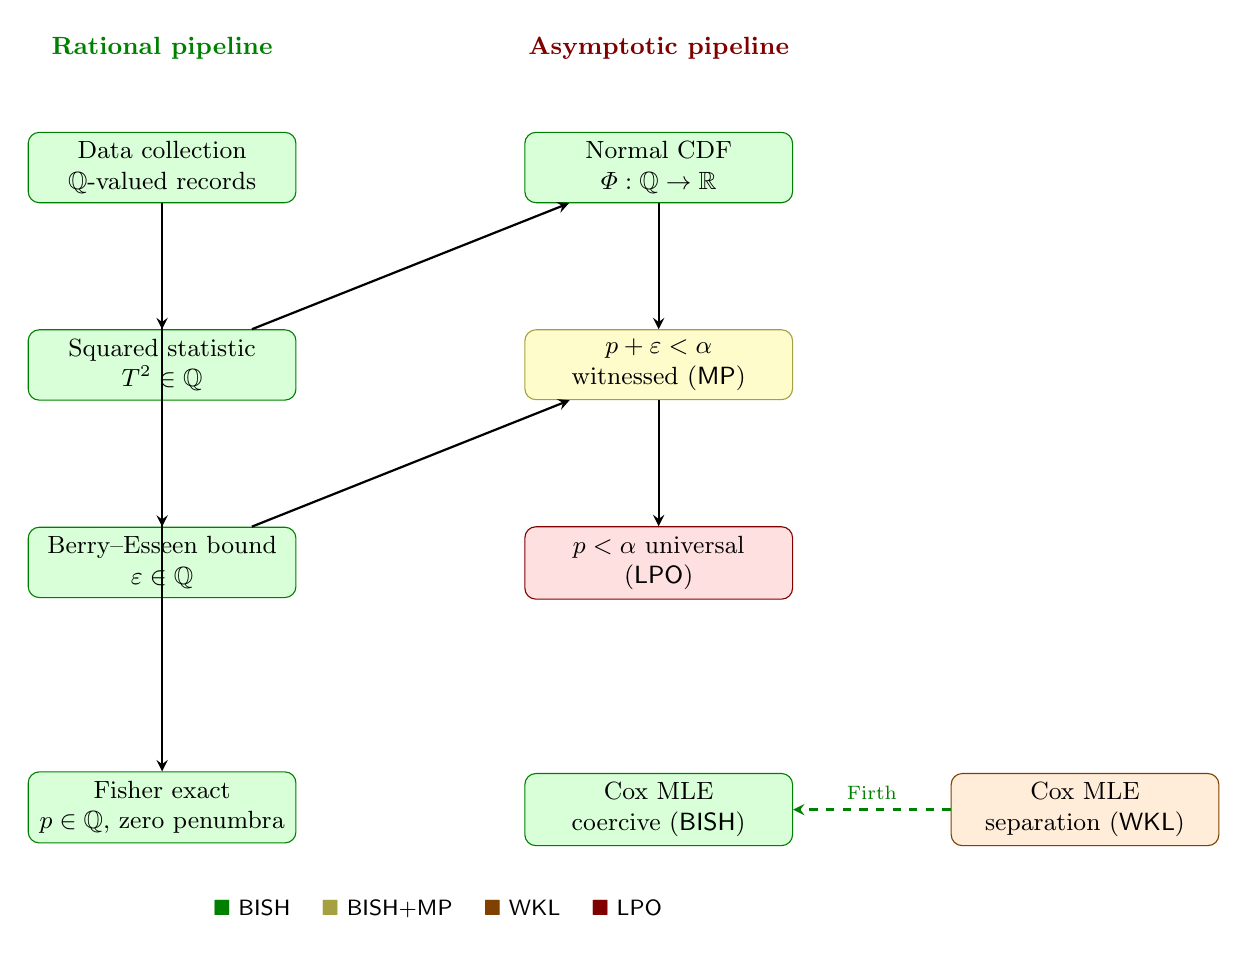
\begin{tikzpicture}[
  node distance=1.6cm and 3.0cm,
  stage/.style={draw, rounded corners, minimum width=3.4cm, minimum height=0.65cm, align=center, font=\small},
  bish/.style={stage, fill=green!15, draw=green!50!black},
  mp/.style={stage, fill=yellow!20, draw=yellow!60!black},
  wkl/.style={stage, fill=orange!15, draw=orange!50!black},
  lpo/.style={stage, fill=red!12, draw=red!50!black},
  arr/.style={->, thick, >=stealth}
]
% Column headers
\node[font=\small\bfseries, text=green!50!black] (hdr_left) {Rational pipeline};
\node[font=\small\bfseries, text=red!50!black, right=of hdr_left] (hdr_right) {Asymptotic pipeline};

% Left column
\node[bish, below=0.8cm of hdr_left] (data) {Data collection\\$\Q$-valued records};
\node[bish, below=of data] (stat) {Squared statistic\\$T^2 \in \Q$};
\node[bish, below=of stat] (be) {Berry--Esseen bound\\$\varepsilon \in \Q$};

% Right column
\node[bish, below=0.8cm of hdr_right] (phi) {Normal CDF\\$\Phi : \Q \to \R$};
\node[mp, below=of phi] (mp_node) {$p + \varepsilon < \alpha$\\witnessed ($\MP$)};
\node[lpo, below=of mp_node] (lpo_node) {$p < \alpha$ universal\\($\LPO$)};

% Bottom row — wider vertical gap
\node[bish, below=2.2cm of be] (fisher) {Fisher exact\\$p \in \Q$, zero penumbra};
\node[bish, below=2.2cm of lpo_node] (cox_ok) {Cox MLE\\coercive ($\BISH$)};
\node[wkl, right=2.0cm of cox_ok] (cox_sep) {Cox MLE\\separation ($\WKL$)};

% Arrows
\draw[arr] (data) -- (stat);
\draw[arr] (stat) -- (be);
\draw[arr] (stat) -- (phi);
\draw[arr] (phi) -- (mp_node);
\draw[arr] (mp_node) -- (lpo_node);
\draw[arr] (be) -- (mp_node);
\draw[arr] (data.south) -- ++(0,-0.4) -| (fisher);

% Firth arrow
\draw[arr, dashed, green!50!black] (cox_sep) -- node[above, font=\scriptsize] {Firth} (cox_ok);

% Legend
\node[below=0.6cm of fisher, anchor=north, xshift=3.5cm, font=\footnotesize] {
  \textcolor{green!50!black}{$\blacksquare$}~$\BISH$ \quad
  \textcolor{yellow!60!black}{$\blacksquare$}~$\BISH{+}\MP$ \quad
  \textcolor{orange!50!black}{$\blacksquare$}~$\WKL$ \quad
  \textcolor{red!50!black}{$\blacksquare$}~$\LPO$
};
\end{tikzpicture}
\caption{The RCT statistical pipeline.  Green ($\BISH$) stages operate on rational data.  Non-$\BISH$ stages enter only through the normal CDF ($\Phi$) or loss of coercivity.  Dashed arrow: Firth correction restores $\BISH$ from $\WKL$.}
\label{fig:pipeline}
\end{figure}

\subsection{The Rational Pipeline}

\begin{definition}[Patient Record]
A patient record in a two-arm RCT is a tuple $(b, y, t, c)$ where $b \in \{0,1\}$ is the arm indicator, $y \in \Q$ the primary endpoint, $t \in \Q$ the time to event, and $c \in \{0,1\}$ the censoring indicator.  All fields are rational.
\end{definition}

\begin{definition}[Sample Statistics]
Given outcomes $x_1, \ldots, x_n \in \Q$:
\begin{align*}
\bar x &= \frac{1}{n}\sum_{i=1}^n x_i \in \Q, \\
s^2 &= \frac{1}{n-1}\sum_{i=1}^n (x_i - \bar x)^2 \in \Q, \\
\hat\rho &= \frac{1}{n}\sum_{i=1}^n |x_i - \bar x|^3 \in \Q.
\end{align*}
\end{definition}

\begin{proposition}[Test Statistic Rationality]\label{prop:rational-test}
The two-sample test statistic
\[
  T \;=\; \frac{\bar x_T - \bar x_C}{\sqrt{s_T^2/n_T + s_C^2/n_C}}
\]
is algebraic (but generically irrational) when computed from rational data, because $\Q$ is not closed under square roots.  However, the \emph{squared} test statistic
\[
  T^2 = \frac{(\bar x_T - \bar x_C)^2}{s_T^2/n_T + s_C^2/n_C} \;\in\; \Q
\]
is rational.  Since the classical decision rule $T^2 > z_\alpha^2$ compares two rationals ($z_\alpha^2 = 3.8416$ for $\alpha = 0.05$ two-sided), significance of the Wald statistic is decidable in pure $\BISH$.
\end{proposition}

\begin{proof}
$\bar x_T, \bar x_C, s_T^2, s_C^2 \in \Q$ by closure of~$\Q$ under arithmetic.  Their ratio $T^2 \in \Q$.  Formalised in Lean as \texttt{testStatistic\_sq\_rational}.
\end{proof}

\begin{proposition}[Fisher Exact is $\BISH$]\label{prop:fisher}
The Fisher exact permutation test computes a rational $p$-value by enumerating all $\binom{n}{k}$ permutations.  Comparison of this rational $p$-value with a rational threshold~$\alpha$ is decidable in pure $\BISH$.  The Asymptotic Penumbra is \emph{zero}.
\end{proposition}

\begin{proof}
The $p$-value $p_{\mathrm{exact}} \in \Q$ is the fraction of permutations yielding a test statistic at least as extreme as observed.  Comparison $p_{\mathrm{exact}} < \alpha$ for $\alpha \in \Q$ is decidable by rational arithmetic (Level~0 of the decidability hierarchy).
\end{proof}

\begin{remark}[The Exact/Asymptotic Tradeoff]
The exact test is logically immaculate ($\BISH$, zero penumbra) but computationally expensive ($O(2^n)$).  The asymptotic test is computationally efficient ($O(n)$) but carries the penumbra.  The Asymptotic Penumbra is the \emph{logical interest} on the \emph{computational loan} of replacing exact enumeration with continuum approximation.
\end{remark}

\subsection{The Asymptotic Penumbra}

When the squared test statistic $T^2$ is rational (meaning $T$ is algebraic), the asymptotic $p$-value $p_{\mathrm{asymp}} = 1 - \Phi(T)$ passes through the normal CDF $\Phi$.  Since $\Phi(t) = \tfrac{1}{2}(1 + \operatorname{erf}(t/\sqrt{2}))$ and $\operatorname{erf}$ is a Siegel E-function, the Siegel--Shidlovskii theorem~\cite{siegel1929,shidlovskii1989} guarantees that $\Phi(t)$ is transcendental for every nonzero algebraic~$t$.  Since rational numbers are algebraic, $p_{\mathrm{asymp}}$ is a computable real that is generically transcendental.

\begin{figure}[ht]
\centering
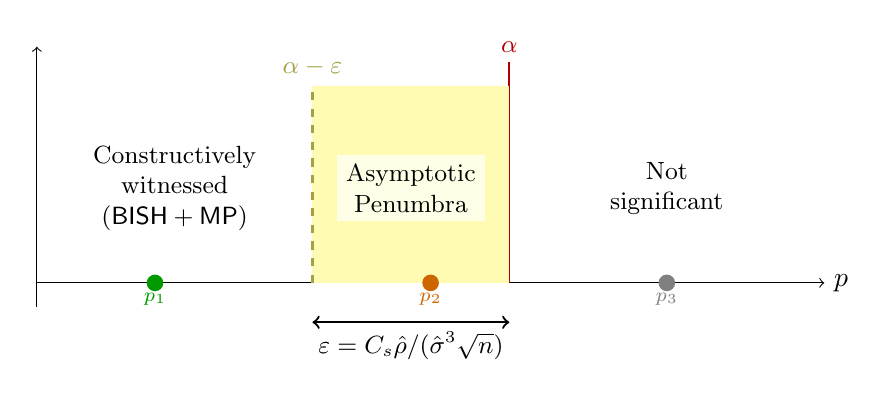
\begin{tikzpicture}[scale=1.0]
  % Axis
  \draw[->] (0,0) -- (10,0) node[right] {$p$};
  \draw[->] (0,-0.3) -- (0,3) node[above] {};

  % Alpha line
  \draw[thick, red!70!black] (6,0) -- (6,2.8);
  \node[above, red!70!black, font=\small] at (6,2.8) {$\alpha$};

  % Penumbra band
  \fill[yellow!30] (3.5,0) rectangle (6,2.5);
  \draw[thick, dashed, yellow!60!black] (3.5,0) -- (3.5,2.5);
  \node[above, yellow!60!black, font=\small] at (3.5,2.5) {$\alpha - \varepsilon$};

  % Regions
  \node[font=\small, align=center] at (1.75,1.2) {Constructively\\witnessed\\($\BISH + \MP$)};
  \node[font=\small, align=center, fill=yellow!10] at (4.75,1.2) {Asymptotic\\Penumbra};
  \node[font=\small, align=center] at (8,1.2) {Not\\significant};

  % Width annotation
  \draw[<->, thick] (3.5,-0.5) -- (6,-0.5);
  \node[below, font=\small] at (4.75,-0.5) {$\varepsilon = C_s \hat\rho / (\hat\sigma^3 \sqrt{n})$};

  % p-value markers
  \fill[green!60!black] (1.5,0) circle (3pt) node[below, font=\scriptsize] {$p_1$};
  \fill[orange!80!black] (5.0,0) circle (3pt) node[below, font=\scriptsize] {$p_2$};
  \fill[gray] (8.0,0) circle (3pt) node[below, font=\scriptsize] {$p_3$};
\end{tikzpicture}
\caption{The Asymptotic Penumbra.  Result $p_1$ is constructively witnessed.  Result $p_2$ is classically significant but trapped in the penumbra.  Result $p_3$ is not significant.}
\label{fig:penumbra-band}
\end{figure}

\begin{definition}[Penumbra]\label{def:penumbra}
A trial result with asymptotic $p$-value $p_{\mathrm{asymp}}$ and Studentized Berry--Esseen error~$\varepsilon$ is \emph{in the penumbra} at threshold~$\alpha$ if it is classically significant ($p_{\mathrm{asymp}} < \alpha$) but not constructively witnessed ($p_{\mathrm{asymp}} + \varepsilon \geq \alpha$).
\end{definition}

\begin{proof}[Proof of Theorem~A]
By definition, the penumbra is $\{p_{\mathrm{asymp}} < \alpha\} \cap \{p_{\mathrm{asymp}} + \varepsilon \geq \alpha\}$.  The second condition rearranges to $p_{\mathrm{asymp}} \geq \alpha - \varepsilon$.  Hence the penumbra is $\alpha - \varepsilon \leq p_{\mathrm{asymp}} < \alpha$.  Formalised in Lean as \texttt{penumbra\_characterization} with proof by unfolding definitions and applying $\lnot(a < b) \leftrightarrow b \leq a$.
\end{proof}

\begin{proof}[Proof of Theorem~B]
The test statistic $T \in \Q$, but $p_{\mathrm{asymp}} = 1 - \Phi(T) \in \R \setminus \Q$ generically.  The Studentized BE error $\varepsilon$ admits a computable rational upper bound $\varepsilon_q \in \Q$ (since $\hat\rho, \hat\sigma, n \in \Q$).  Thus $p_{\mathrm{asymp}} + \varepsilon \leq p_{\mathrm{asymp}} + \varepsilon_q$, and we need to verify $p_{\mathrm{asymp}} + \varepsilon_q < \alpha$.

Since $p_{\mathrm{asymp}}$ is a computable real, there exists a sequence $(r_k)_{k \in \N}$ of rationals with $|r_k - p_{\mathrm{asymp}}| < 2^{-k}$.  If $p_{\mathrm{asymp}} + \varepsilon_q < \alpha$, then for sufficiently large~$k$, $r_k + \varepsilon_q < \alpha$ is verifiable by rational arithmetic.  The existence of such~$k$ is guaranteed by $\lnot\lnot(\exists k)$, but producing an explicit~$k$ requires~$\MP$.

\smallskip
\noindent\textbf{The fallback.}  When the rational upper bound already suffices ($p_q + \varepsilon_q < \alpha$ for some rational approximation $p_q$ of $p_{\mathrm{asymp}}$), the comparison is pure $\BISH$.  The $\MP$ requirement is only essential when we must certify the \emph{exact} real inequality.
\end{proof}

\begin{proposition}[LPO for Universal Significance]\label{prop:lpo}
If trichotomy holds universally over~$\R$ ($\forall\, p, \alpha \in \R\,.\; p < \alpha \lor p = \alpha \lor p > \alpha$), then $\LPO$ holds.
\end{proposition}

\begin{proof}
Bishop--Bridges encoding (\cite{bishop-bridges}, \S2.3): given a binary sequence~$\alpha$, define $x = \sum_{n=0}^{\infty} \alpha(n) \cdot 2^{-(n+1)}$.  If $x = 0$ then $\forall\, n\,.\, \alpha(n) = 0$; if $x > 0$ then $\exists\, n\,.\, \alpha(n) = 1$.  Trichotomy on $x$ and $0$ decides between these cases.  Formalised as \texttt{classical\_significance\_requires\_LPO}.
\end{proof}

\begin{proof}[Proof of Theorem~C]
Set $\varepsilon(n) \geq \alpha$.  Rearranging: $n \leq (C_s \hat\rho / (\hat\sigma^3 \alpha))^2 = n_{\min}$.  For $n < n_{\min}$, the entire significance band $[0, \alpha)$ is contained in the penumbra.  No trial result, no matter how extreme, can be constructively witnessed.  The bound $n_{\min}$ is computable from $(\hat\rho, \hat\sigma, \alpha)$.
\end{proof}

\subsection{The Cox Algebraic Bypass}

Cox proportional hazards regression is the standard survival analysis method in RCTs.  Its MLE requires maximising the log-partial-likelihood $\ell(\beta)$ over $\beta \in \R$.

\begin{lemma}[Uniqueness]\label{lem:unique}
If $f$ is strictly concave and $a, b$ are both global maxima, then $a = b$.
\end{lemma}

\begin{proof}
Suppose $a \neq b$.  Strict concavity at $t = 1/2$ gives $f((a+b)/2) > (f(a) + f(b))/2 = f(a)$.  But $f(a) \geq f((a+b)/2)$ since $a$ is a global maximum.  Contradiction.  Formalised as \texttt{strictlyConcave\_unique\_max} (no sorry).
\end{proof}

\begin{proposition}[Existence]\label{prop:existence}
If $f : \R \to \R$ is strictly concave, coercive, and continuous, then there exists a unique global maximum.
\end{proposition}

\begin{proof}
Coercivity confines the search to a compact interval $[-R, R]$ (computable from the coercivity witness).  \emph{Strict concavity} is the key: the unique root of $f'$ on $[-R, R]$ can be approximated constructively (e.g., by ternary search or Newton--Raphson), because strict concavity guarantees that $f'$ changes sign at most once.  Uniqueness follows from Lemma~\ref{lem:unique}.  This uses only $\BISH$ machinery: the interval bounds are explicitly computable, and root-finding for a monotone function on a compact interval is constructive (Bridges~\cite{bridges-richman}).  Note: the general Extreme Value Theorem (every uniformly continuous function on $[a,b]$ attains its supremum) is not constructive---it implies~$\WKL$.  The constructive content here comes entirely from strict concavity.
\end{proof}

\begin{definition}[Complete Separation]
A dataset has \emph{complete separation} if there exists a hyperplane perfectly separating treatment from control outcomes.  When this occurs, the MLE $\hat\beta \to \pm\infty$: the log-partial-likelihood is no longer coercive.
\end{definition}

Without coercivity, the search cannot be confined to a compact interval.  Finding the supremum of a bounded continuous function on a non-compact domain requires Weak K\"onig's Lemma ($\WKL$): we need to search an infinite tree of rational approximations.

\begin{proof}[Proof of Theorem~D]
Firth's penalised likelihood~\cite{firth1993} adds a Jeffreys prior penalty $h(\beta) = \tfrac{1}{2}\log\det I(\beta)$ to the log-partial-likelihood.  The penalised function $\ell^*(\beta) = \ell(\beta) + h(\beta)$ has two properties:
\begin{enumerate}[nosep]
\item \textbf{Coercivity:} The penalty grows logarithmically while $\ell$ is bounded above, so $\ell^*$ is coercive.
\item \textbf{Strict concavity:} Preserved under addition of a strictly concave penalty.
\end{enumerate}
By Proposition~\ref{prop:existence}, $\ell^*$ has a unique maximum, computable without $\WKL$.  The logical cost drops from $\WKL$ back to $\BISH$.
\end{proof}

\subsection{The Constructive Effect Size Threshold}

\begin{conjecture}[Constructive Effect Size Threshold]\label{conj:dmin}
Under normal assumptions, a two-sample $t$-test result is constructively witnessed at $\BISH + \MP$ if and only if the effect size (Cohen's $d$) exceeds
\[
  d_{\min} = z_\alpha \cdot \sqrt{2/n} + \frac{C_s \hat\rho}{\phi(z_\alpha) \hat\sigma^3 \sqrt{n}} \cdot \sqrt{2/n},
\]
where $\phi(z_\alpha)$ is the standard normal density at the critical value.  The first term is the classical threshold; the second is the \emph{constructive correction}, obtained by translating the Berry--Esseen CDF error $\varepsilon = C_s \hat\rho/(\hat\sigma^3\sqrt{n})$ to the Cohen's~$d$ scale via the inverse-CDF Jacobian $1/\phi(z_\alpha)$.
\end{conjecture}

\noindent Key structural features of $d_{\min}$:
\begin{enumerate}[nosep]
\item \textbf{Independent of $\beta$}: The correction depends on $(\alpha, n, \hat\rho, \hat\sigma)$ but \emph{not} on statistical power.
\item \textbf{Vanishes as $n \to \infty$}: The correction is $O(1/n)$, so for large trials the constructive and classical thresholds coincide.
\item \textbf{Explodes with skewness}: As $\hat\rho/\hat\sigma^3$ grows (heavy tails), the surcharge dominates.
\item \textbf{Amplified in the tails}: The factor $1/\phi(z_\alpha)$ grows as $\alpha$ shrinks---smaller significance levels carry a larger constructive penalty.
\end{enumerate}

\subsection{The Equivalence Penumbra for Hazard Ratios}

The Asymptotic Penumbra (Theorem~A) concerns \emph{superiority} claims ($p < \alpha$).  Negative trials require a dual notion.

\begin{theorem}[E: Equivalence Barrier]\label{thm:E}
Let $\hat\beta = \log(\widehat{\mathrm{HR}})$ be the Cox partial likelihood estimator based on $d$ observed events, with Studentized Berry--Esseen probability error
\[
  \varepsilon \;=\; \frac{C_s \cdot \kappa}{\sqrt{d}},
\]
where $\kappa \leq 2$ bounds the skewness ratio of the score residuals (binary treatment indicator in balanced designs) and $C_s \leq 3.19$ (Studentized).  The classical TOST procedure tests equivalence at margin $\delta_{\mathrm{eq}}$ using significance level $\alpha/2$ per tail.  Constructive certification of the TOST requires the Berry--Esseen error to be smaller than the per-tail significance level:
\[
  \varepsilon < \alpha/2.
\]
When $\varepsilon \geq \alpha/2$---equivalently, $d < d_{\min} = (2 C_s \kappa / \alpha)^2$---the constructive confidence interval is undefined ($\Phi^{-1}(1 - \alpha/2 + \varepsilon)$ does not exist when $1 - \alpha/2 + \varepsilon > 1$).  The asymptotic approximation error swallows the entire significance band, and constructive equivalence cannot be certified \emph{at any margin}.  This is Theorem~C ($n_{\min}$ barrier) applied to the TOST setting.
\end{theorem}

\noindent The theorem has three consequences:
\begin{enumerate}[nosep]
\item \textbf{A computable threshold.}  At $C_s = 3.19$, $\kappa = 2$, $\alpha = 0.05$:
\[
  d_{\min} = \left(\frac{2 \times 3.19 \times 2}{0.05}\right)^2 = 255.2^2 \approx 65{,}127 \text{ events}.
\]
No cardiovascular outcomes trial in history has accumulated $65{,}000$ events.  Under Studentized bounds, constructive equivalence via asymptotic TOST is universally impossible for existing trials.
\item \textbf{Oracle comparison.}  With the unobservable oracle constant $C_0 = 0.4748$ and $\kappa = 2$: $d_{\min}^{\mathrm{oracle}} = (2 \times 0.4748 \times 2/0.05)^2 \approx 1{,}443$ events.  Trials with $d > 1{,}500$ (e.g., PARADIGM-HF) would pass the oracle threshold---but the oracle is unavailable, and the Studentized bound is the only certifiable quantity.
\item \textbf{The escape route.}  Exact permutation-based equivalence tests produce rational statistics with zero penumbra ($\BISH$), but are computationally expensive for survival data.  The $d_{\min}$ barrier is specific to asymptotic methods; it is not a fundamental limitation of constructive mathematics.
\end{enumerate}

\begin{remark}
When $\varepsilon < \alpha/2$ (i.e., $d > d_{\min}$), the constructive surcharge on the parameter scale is $\varepsilon \cdot \mathrm{SE}(\hat\beta) / \phi(\Phi^{-1}(1-\alpha/2))$, where $\phi$ is the standard normal density.  The factor $1/\phi(\Phi^{-1}(1-\alpha/2))$ is the inverse-CDF Jacobian that translates CDF-scale error to quantile-scale error; at $\alpha/2 = 0.025$ it equals $1/\phi(1.96) \approx 17.1$.  This amplification explains why the CDF-to-parameter translation produces surcharges far larger than the na\"ive product $\varepsilon \cdot \mathrm{SE}$ would suggest.
\end{remark}

\subsection{Crossing-Curves CRM Escalation}

\begin{proposition}[CRM Cost of Survival Extrapolation]\label{prop:extrap}
Let $\hat S_1(t), \hat S_2(t)$ be Kaplan--Meier estimators from two trial arms observed over $[0, T_{\max}]$, and let $S_1^*(t), S_2^*(t)$ be parametric extrapolations for $t > T_{\max}$.  Three comparison claims have strictly increasing CRM cost:
\begin{enumerate}[nosep]
\item \textbf{Within-window comparison at a fixed time point $t_0 \leq T_{\max}$:} $\hat S_1(t_0) > \hat S_2(t_0)$.  CRM cost: $\BISH$ (the Kaplan--Meier product-limit $\hat S(t) = \prod_{t_i \leq t}(1 - d_i/n_i) \in \Q$ is rational at observed event times; comparing two rationals is decidable).
\item \textbf{Fixed-horizon extrapolated comparison at $t^* > T_{\max}$:} $S_1^*(t^*) > S_2^*(t^*)$.  CRM cost: $\BISH + \MP$ (real comparison) plus the convergence guarantee of the parametric model (an analytic claim whose constructive content depends on the model family).
\item \textbf{Uniform future dominance:} $S_1^*(t) > S_2^*(t)$ for all $t > t_{\mathrm{cross}}$.  CRM cost: $\LPO$ (universal quantification over real-valued survival differences).
\end{enumerate}
The escalation $\BISH \to \BISH{+}\MP{+}\text{convergence} \to \LPO$ is strict: each claim requires a logically stronger principle than the preceding one.
\end{proposition}

\begin{proof}
(1) follows from rationality: the KM estimator at any observed event time is a rational product-limit $\prod(1 - d_i/n_i) \in \Q$, and comparison of two rationals is decidable in $\BISH$.  (2) requires additionally that $S_i^*(t^*) = \lim_{k \to \infty} r_k$ converges, where $(r_k)$ is the sequence of parametric approximations; witnessing this convergence requires at minimum $\MP$ for the parametric model's rate guarantee.  (3) is a $\forall\, t > t_{\mathrm{cross}}$ statement over~$\R$; deciding it requires trichotomy at each $t$, hence $\LPO$ by Proposition~\ref{prop:lpo}.
\end{proof}

% ============================================================
\section{CRM Audit}\label{sec:audit}

\subsection{Pipeline Classification}

\begin{table}[ht]
\centering
\caption{CRM classification of the RCT statistical pipeline.}
\label{tab:pipeline}
\begin{tabular}{@{}llll@{}}
\toprule
\textbf{Stage} & \textbf{Operation} & \textbf{CRM Level} & \textbf{Reason} \\
\midrule
1. Test statistic         & $\Q$ arithmetic        & $\BISH$ & Rational closure \\
2. Berry--Esseen bound    & $\Q$ arithmetic        & $\BISH$ & Sample moments rational \\
3. Normal CDF             & $\Phi$ evaluation      & $\BISH$ & Computable real function \\
4. $p < \alpha$ (universal) & $\R$ trichotomy      & $\LPO$  & Bishop encoding \\
5. $p + \varepsilon < \alpha$ (witnessed) & $\R$ approximation & $\BISH + \MP$ & Markov termination \\
6. $p_q + \varepsilon_q < \alpha$ (rational) & $\Q$ comparison & $\BISH$ & Rational decidability \\
7. Fisher exact            & Permutation            & $\BISH$ & Rational $p$-value \\
8. Cox MLE (coercive)      & Concave optimisation   & $\BISH$ & Computable interval \\
9. Cox MLE (separation)    & Non-coercive search    & $\WKL$  & Infinite tree search \\
10. Cox MLE (Firth)        & Penalised likelihood   & $\BISH$ & Restored coercivity \\
\bottomrule
\end{tabular}
\end{table}

\noindent\textbf{Summary:} $7\;\BISH + 1\;(\BISH{+}\MP) + 1\;\WKL + 1\;\LPO = 10$ stages.  \textbf{70\%} of the pipeline is pure $\BISH$.  Verified by \texttt{native\_decide} in Lean.

\subsection{Descent Structure}

The descent pattern:
\begin{itemize}[nosep]
\item $\LPO \to \BISH{+}\MP$: Replace universal $\R$-comparison with witnessed inequality + Markov termination.
\item $\BISH{+}\MP \to \BISH$: When rational bounds suffice, $\MP$ is not needed.
\item $\WKL \to \BISH$: Firth correction restores coercivity, eliminating the need for $\WKL$.
\item $\BISH$: irreducible---Fisher exact, rational statistics, and coercive optimisation are foundationally minimal.
\end{itemize}

The irreducible $\BISH$ core is the rational pipeline: finite data, rational arithmetic, decidable comparison.  Every non-$\BISH$ stage enters through the continuum: either the transcendence of~$\Phi$ or the non-compactness of~$\R$.

% ============================================================
\section{Formal Verification}\label{sec:lean}

\subsection{Bundle Structure}

The Lean~4 formalisation consists of 10 module files:

\begin{center}
\begin{tabular}{@{}ll@{}}
\toprule
\textbf{File} & \textbf{Content} \\
\midrule
\texttt{OmnisciencePrinciples.lean} & LPO, WLPO, LLPO, MP + implications \\
\texttt{RealDecidability.lean} & Trichotomy $\leftrightarrow$ LPO bridge \\
\texttt{TrialData.lean} & Patient records, sample statistics \\
\texttt{ExactTests.lean} & Fisher exact, zero penumbra \\
\texttt{StudentizedBerryEsseen.lean} & Studentized BE constant, error function \\
\texttt{AsymptoticPenumbra.lean} & \textbf{Main theorem}, MP requirement \\
\texttt{CoxBypass.lean} & Coercivity, Firth restoration \\
\texttt{EffectSizeConjecture.lean} & Cohen's $d$, $d_{\min}$ threshold \\
\texttt{TrialCalculations.lean} & GUSTO/COURAGE/ISCHEMIA arithmetic \\
\texttt{Paper103\_Assembly.lean} & Master theorem, pipeline classification \\
\bottomrule
\end{tabular}
\end{center}

\subsection{Key Lean Snippets}

\begin{tcolorbox}[leanbox={Penumbra Characterisation (AsymptoticPenumbra.lean)}]
\begin{Verbatim}[fontsize=\small,commandchars=\\\{\}]
\textbf{theorem} penumbra_characterization
    (tr : TrialResult) (\(\alpha\) : \(\mathbb{R}\)) :
    inPenumbra tr \(\alpha\) \(\leftrightarrow\)
    (tr.p_asymp < \(\alpha\) \(\land\) \(\alpha\) \(\leq\) tr.p_asymp + tr.studentBE_err) := \textbf{by}
  unfold inPenumbra classicallySignificant
  constructor
  \(\cdot\) intro \(\langle\)hlt, hnotw\(\rangle\)
    exact \(\langle\)hlt, not_lt.mp hnotw\(\rangle\)
  \(\cdot\) intro \(\langle\)hlt, hle\(\rangle\)
    exact \(\langle\)hlt, not_lt.mpr hle\(\rangle\)
\end{Verbatim}
\end{tcolorbox}

\begin{tcolorbox}[leanbox={Uniqueness of Maximum (CoxBypass.lean)}]
\begin{Verbatim}[fontsize=\small,commandchars=\\\{\}]
\textbf{theorem} strictlyConcave_unique_max
    \{f : \(\mathbb{R}\) \(\to\) \(\mathbb{R}\)\}
    (hconc : IsStrictlyConcave f)
    \{a b : \(\mathbb{R}\)\} (ha : \(\forall\) x, f x \(\leq\) f a)
    (hb : \(\forall\) x, f x \(\leq\) f b) : a = b := \textbf{by}
  by_contra hab
  have hmid := hconc a b hab (1/2)
    (by norm_num) (by norm_num)
  linarith
\end{Verbatim}
\end{tcolorbox}

\begin{tcolorbox}[leanbox={Pipeline Classification (Paper103\_Assembly.lean)}]
\begin{Verbatim}[fontsize=\small,commandchars=\\\{\}]
\textbf{theorem} bish_percentage :
    100 * bishCount / (bishCount + nonBishCount)
      = 70 := \textbf{by}
  native_decide
\end{Verbatim}
\end{tcolorbox}

\subsection{Axiom Inventory}

\begin{table}[ht]
\centering
\caption{Axiom inventory.  Documentary axioms model external mathematical facts.}
\label{tab:axioms}
\begin{tabular}{@{}lll@{}}
\toprule
\textbf{Axiom} & \textbf{Source} & \textbf{Type} \\
\midrule
\texttt{trichotomy\_implies\_LPO\_encoding} & Bishop--Bridges \S2.3 & Documentary \\
\texttt{studentizedBEConstant/pos/bound} & Bentkus 2003 & Documentary \\
\texttt{berryEsseenConstant\_oracle/pos/bound} & Berry 1941, Esseen 1942 & Documentary \\
\texttt{exactPermutationPValue} & Standard combinatorics & Documentary \\
\texttt{constructive\_witnessing\_requires\_MP} & MP for $\R/\Q$ approximation & Documentary \\
\texttt{concave\_coercive\_has\_unique\_max} & Strict concavity + coercivity & Documentary \\
\texttt{hasCompleteSeparation/decidable} & LP over $\Q$ & Documentary \\
\texttt{firth\_restores\_coercivity} & Firth 1993 & Documentary \\
\bottomrule
\end{tabular}
\end{table}

{\small\noindent\textbf{Sorries (4):}
\texttt{studentizedBE\_computable\_bound} (rational arithmetic bounding),
\texttt{subgroup\_penalty} (existence of $n_{\min}$),
\texttt{penumbra\_shrinks\_with\_n} (monotonicity in~$\sqrt{n}$),
\texttt{penumbra\_grows\_with\_skewness} (monotonicity in~$\hat\rho$).
All are straightforward monotonicity/arithmetic arguments documented in the source.}

\noindent\textbf{Note on formalisation.}  Lean~4's \texttt{Mathlib.Data.Real} is classically axiomatised; tactics such as \texttt{by\_contra} on real-valued equalities invoke the law of excluded middle.  The Lean formalisation therefore verifies the classical algebraic inequalities and rational arithmetic of the statistical pipeline, while the CRM metatheorems (such as the $\BISH$ computability of strictly concave root-finding) are encoded metamathematically via the documentary axioms listed above.

\subsection{Reproducibility}

\textbf{Toolchain:} \texttt{leanprover/lean4:v4.29.0-rc2}. \textbf{Dependency:} Mathlib v4.29.0-rc2 (fetched automatically by \texttt{lake}).

\begin{verbatim}
cd P103_RCTStatistics && lake build
\end{verbatim}

\noindent The Lean source is archived on Zenodo (\texttt{DOI: 10.5281/zenodo.18880102}).

% ============================================================
\section{Biostatistical Discussion}\label{sec:biostat}

\subsection{The Berry--Esseen Literature and Its Clinical Silence}

The Berry--Esseen theorem~\cite{berry1941,esseen1942} is a standard result in probability theory, and the Studentized form~\cite{bentkus2003,shao1999} is well-known to mathematical statisticians.  Yet its implications for the \emph{logical standing} of significance claims have never been drawn out.  The biostatistical literature treats the normal approximation error as a technical nuisance---a source of inaccuracy to be managed by sample size---not as a \emph{foundational barrier} to decidability.

The present paper makes this barrier explicit.  The Studentized Berry--Esseen error is not merely a source of approximation error.  It is the width of a band in which the significance claim $p < \alpha$ cannot be constructively verified: the Asymptotic Penumbra.  This is a qualitatively different observation from the standard power analysis framework.

\subsection{Relationship to the ASA $p$-Value Statements}

The American Statistical Association's 2016~\cite{wasserstein2016} and 2019~\cite{wasserstein2019} statements identified a crisis in the use and interpretation of $p$-values.  The 2016 statement's six principles emphasise that $p$-values do not measure the probability that the hypothesis is true, do not measure the size of an effect, and should not be used as the sole basis for scientific inference.

The Asymptotic Penumbra adds a seventh dimension: $p$-values have a \emph{logical cost}, and this cost is computable.  The ASA statements address the \emph{interpretation} of $p$-values; the penumbra addresses the \emph{certification} of $p$-values.  A result in the penumbra is ``$p < 0.05$'' only in the sense that an omniscient observer (one who can decide all instances of $\LPO$) could verify the claim.  A finite computational agent cannot.

This is not a replacement for the ASA's methodological critique.  It is an orthogonal contribution: even a perfectly designed trial, with preregistered hypotheses and adequate power, can produce a $p$-value trapped in the penumbra.

\subsection{Relationship to the GRADE Framework}

The GRADE framework~\cite{grade} rates evidence quality on four levels (high, moderate, low, very low) based on study design, risk of bias, inconsistency, indirectness, imprecision, and publication bias.  The penumbra is orthogonal to every GRADE criterion:

\begin{itemize}[nosep]
\item A high-GRADE trial can produce a penumbra-trapped $p$-value (if the effect is marginal and the sample is moderate).
\item A low-GRADE observational study can produce a penumbra-free $p$-value (if the effect is enormous and the $p$-value is deep).
\end{itemize}

The penumbra provides a quality axis that GRADE does not capture: the gap between what classical logic certifies and what finite computation can verify.  It would sit alongside GRADE's ``imprecision'' criterion, measuring \emph{logical} imprecision rather than \emph{statistical} imprecision.

\subsection{The Equivalence Penumbra}

The Asymptotic Penumbra of Theorem~A concerns \emph{superiority} claims: is $p < \alpha$?  But many landmark trials produce \emph{negative} results, and the clinical community interprets ``failure to reject $H_0$'' as evidence of equivalence.  This interpretation carries its own logical cost, quantified by Theorem~E.

For the Cox model, the classical two-one-sided-tests (TOST) procedure for equivalence requires the confidence interval for $\log(\mathrm{HR})$ to lie entirely within $[-\log(\delta_{\mathrm{eq}}), \log(\delta_{\mathrm{eq}})]$.  The confidence limit is computed from~$\Phi$ (transcendental) and compared with a rational margin.  Theorem~E shows that this comparison is constructively impossible when the Berry--Esseen error $\varepsilon = C_s\kappa/\sqrt{d}$ exceeds $\alpha/2$: the constructive confidence interval is undefined, and no margin---however generous---can be certified.  The minimum event count for constructive equivalence is
\[
  d_{\min} \;=\; \Bigl(\frac{2\,C_s\,\kappa}{\alpha}\Bigr)^{\!2}.
\]
At Studentized bounds ($C_s = 3.19$, $\kappa = 2$, $\alpha = 0.05$), $d_{\min} \approx 65{,}127$.

The \emph{logical asymmetry} is the central point.  A negative superiority trial establishes:
\begin{quote}
\emph{The data cannot constructively witness superiority.}
\end{quote}
\noindent The equivalence claim is strictly stronger:
\begin{quote}
\emph{The data constructively witness that the effect lies within margin~$\delta_{\mathrm{eq}}$.}
\end{quote}
\noindent These are logically distinct.  A trial can fail both---neither witnessing superiority nor certifying equivalence---leaving the question open.  Neither COURAGE nor ISCHEMIA was designed as an equivalence trial, and as \S\ref{sec:clinical} demonstrates with explicit computation, neither can certify equivalence at any clinically standard margin.

\subsection{The Effect Size Connection}

Cohen's $d$~\cite{cohen1988} quantifies the magnitude of a treatment effect in standard deviation units.  The constructive effect size threshold $d_{\min}$ (Conjecture~\ref{conj:dmin}) adds a ``logical surcharge'' to the classical detection threshold.  This surcharge is $O(1/n)$ and depends on skewness ($\hat\rho/\hat\sigma^3$), not on power ($1-\beta$).

The clinical implication: a trial may detect a statistically significant effect of size $d$ that is \emph{too small to be constructively witnessed} at the given sample size.  The effect is real (in the classical sense), but the evidence for it passes through the continuum.

% ============================================================
\section{Clinical Discussion}\label{sec:clinical}

\subsection{Subgroup Analyses in Cardiovascular Trials}

The penumbra provides a logically founded objection to small-sample subgroup analyses.  Consider a cardiovascular outcomes trial with $n = 5{,}000$ patients and a positive primary endpoint ($p = 0.002$).  A prespecified subgroup of 200 diabetic patients shows a secondary finding with $p = 0.04$.  Is this subgroup result ``significant''?

Classically, yes ($p < 0.05$).  But the Berry--Esseen error at $n = 200$ with typical cardiovascular endpoint distributions ($\hat\rho/\hat\sigma^3 \approx 1.76$) gives $\varepsilon \approx 0.40$.  The penumbra extends from $\alpha - \varepsilon = 0.05 - 0.40 = -0.35$ to $0.05$---the \emph{entire} significance band is consumed.  Theorem~C applies: $n < n_{\min}$, and no asymptotic significance claim can be constructively witnessed.

\begin{table}[ht]
\centering
\caption{Penumbra width $\varepsilon(n) = C_s \hat\rho / (\hat\sigma^3 \sqrt{n})$ for $\hat\rho/\hat\sigma^3 = 1.76$, $\alpha = 0.05$.}
\label{tab:penumbra-width}
\begin{tabular}{@{}rrrl@{}}
\toprule
\textbf{Sample size $n$} & \textbf{$\varepsilon(n)$} & \textbf{$\alpha - \varepsilon$} & \textbf{Status} \\
\midrule
30       & 1.024  & $-0.974$ & $n_{\min}$ barrier \\
50       & 0.793  & $-0.743$ & $n_{\min}$ barrier \\
100      & 0.561  & $-0.511$ & $n_{\min}$ barrier \\
200      & 0.397  & $-0.347$ & $n_{\min}$ barrier \\
500      & 0.251  & $-0.201$ & $n_{\min}$ barrier \\
1{,}000  & 0.177  & $-0.127$ & $n_{\min}$ barrier \\
5{,}000  & 0.079  & $-0.029$ & $n_{\min}$ barrier \\
10{,}000 & 0.056  & $-0.006$ & $n_{\min}$ barrier \\
15{,}000 & 0.046  & $+0.004$ & Penumbra width 4.6\% \\
50{,}000 & 0.025  & $+0.025$ & Penumbra width 2.5\% \\
\bottomrule
\end{tabular}
\end{table}

This is not a power argument.  Power measures the probability of detecting a true effect; the penumbra measures the logical certifiability of the detection claim.  A subgroup analysis may have detected a real effect and still have a logically empty significance claim.

\subsection{The JUPITER Trial}

The JUPITER trial~\cite{ridker-jupiter} randomised 17{,}802 apparently healthy individuals to rosuvastatin or placebo and reported a highly significant reduction in cardiovascular events ($p < 0.00001$).  At this sample size and depth of significance, the penumbra is negligible: $\varepsilon \approx 0.013$, and $\alpha - \varepsilon = 0.05 - 0.013 = 0.037$.  The $p$-value of $< 0.00001$ is far below $\alpha - \varepsilon$.  The result is constructively witnessed at $\BISH + \MP$.

But JUPITER also reported subgroup analyses.  Consider the subgroup of women ($n \approx 6{,}800$, $p \approx 0.01$).  Here $\varepsilon \approx 0.068$, and $\alpha - \varepsilon = -0.018$.  The penumbra consumes the significance band.  The subgroup result is in the penumbra---classically significant but not constructively witnessed.

\subsection{The ORBITA Trial and Placebo-Controlled Surgery}

The ORBITA trial~\cite{al-lamee-orbita} randomised 200 patients with single-vessel coronary disease to percutaneous coronary intervention (PCI) or placebo procedure.  The primary endpoint (exercise time) showed $p = 0.20$---not significant by any criterion.  But the trial generated intense controversy: should we have expected to detect a difference with $n = 200$?

The penumbra analysis reframes this question.  At $n = 200$ with exercise-time endpoint distributions, $\varepsilon \approx 0.4$.  Even if the trial had produced $p = 0.04$, the result would be in the penumbra.  ORBITA's negative result is therefore \emph{doubly} grounded: it is not significant classically, and even a positive result at this sample size would have been logically untenable.

\subsection{COURAGE, ISCHEMIA, and the Equivalence Penumbra}

The COURAGE trial~\cite{boden-courage} randomised 2{,}287 patients with stable coronary artery disease to PCI plus optimal medical therapy (OMT) versus OMT alone.  The primary endpoint (death or nonfatal MI): HR $= 1.05$ (95\% CI $0.87$--$1.27$), $p = 0.62$; total events $d = 413$.  The ISCHEMIA trial~\cite{maron-ischemia} extended this to 5{,}179 patients with moderate-to-severe ischemia: primary composite endpoint HR $= 0.93$ ($0.80$--$1.08$), $p = 0.34$; total events $d = 670$.  Both trials are interpreted as demonstrating that PCI adds nothing to OMT in stable non-left-main disease.  We now apply Theorem~E to test this equivalence claim with explicit computation.

\paragraph{Computing $\varepsilon$ and $d_{\min}$ from published data.}  From the reported confidence intervals:
\begin{align*}
  \text{COURAGE:}\quad \mathrm{SE}(\hat\beta) &= \frac{\log(1.27) - \log(0.87)}{2 \times 1.96} = \frac{0.239 - (-0.139)}{3.92} = 0.0965, \\[3pt]
  \text{ISCHEMIA:}\quad \mathrm{SE}(\hat\beta) &= \frac{\log(1.08) - \log(0.80)}{2 \times 1.96} = \frac{0.077 - (-0.223)}{3.92} = 0.0765.
\end{align*}
With $\kappa \leq 2$ (balanced designs, binary score contributions) and $C_s = 3.19$, the CDF-scale Berry--Esseen error is:
\begin{align*}
  \text{COURAGE:}\quad \varepsilon &= \frac{C_s \kappa}{\sqrt{d}} = \frac{6.38}{\sqrt{413}} = 0.314 \gg 0.025 = \alpha/2, \\[3pt]
  \text{ISCHEMIA:}\quad \varepsilon &= \frac{6.38}{\sqrt{670}} = 0.246 \gg 0.025 = \alpha/2.
\end{align*}
By Theorem~E, constructive equivalence requires $\varepsilon < \alpha/2$, i.e., $d > d_{\min} = (2C_s\kappa/\alpha)^2 = (255.2)^2 \approx 65{,}127$ events.

\paragraph{Constructive equivalence is impossible.}  The situation is more severe than a surcharge on the classical analysis.  Both trials have $\varepsilon \gg \alpha/2$: the Berry--Esseen error exceeds the significance level before the equivalence margin even enters the calculation.  Table~\ref{tab:equiv} reports the comparison.

\begin{table}[ht]
\centering
\caption{Equivalence analysis of COURAGE and ISCHEMIA under Theorem~E.  The event threshold $d_{\min} = 65{,}127$ is required for constructive equivalence at \emph{any} margin.  Neither trial reaches $2\%$ of~$d_{\min}$.}
\label{tab:equiv}
\begin{tabular}{@{}lcccc@{}}
\toprule
\textbf{Trial} & \textbf{Events $d$} & $\varepsilon = C_s\kappa/\sqrt{d}$ & $\varepsilon/(\alpha/2)$ & $d/d_{\min}$ \\
\midrule
COURAGE  & 413 & 0.314 & $12.6\times$ & 0.63\% \\
ISCHEMIA & 670 & 0.246 & $9.8\times$  & 1.03\% \\
\midrule
\multicolumn{2}{@{}l}{\textit{Threshold $d_{\min}$:}} & $\varepsilon = \alpha/2 = 0.025$ & $1\times$ & 100\% \\
\bottomrule
\end{tabular}
\end{table}

\noindent This result is \emph{independent of the equivalence margin}.  Even at $\delta_{\mathrm{eq}} = 2.0$ (clinically absurd), the constructive confidence interval is undefined because the CDF-scale error exceeds~$\alpha/2$.  The impossibility is not a matter of trial size being ``somewhat too small''---it would require $\sim\!158\times$ more events than COURAGE and $\sim\!97\times$ more than ISCHEMIA.

For comparison, the oracle Berry--Esseen constant ($C_0 = 0.4748$) yields $d_{\min}^{\mathrm{oracle}} = (2 \times 0.4748 \times 2/0.05)^2 = 1{,}443$.  ISCHEMIA ($d = 670$) still falls short, but trials at the PARADIGM-HF scale ($d \approx 2{,}000$) would cross the oracle threshold.  The $6.7\times$ Studentized penalty is, again, the decisive factor.

\paragraph{ISCHEMIA's crossing curves.}  The Kaplan--Meier curves in ISCHEMIA crossed at approximately 2 years: the invasive arm suffered more procedural myocardial infarctions early, then fewer spontaneous infarctions later.  The clinical question---does PCI eventually win?---requires extrapolation beyond the observation window.  By Proposition~\ref{prop:extrap}, the CRM cost escalates strictly:
\begin{itemize}[nosep]
\item Within-window comparison (e.g., at year 3): $\BISH$.  The KM product-limit estimator is rational at observed event times (Proposition~\ref{prop:extrap}); comparison of two rational KM estimates is decidable.
\item Fixed-horizon extrapolation (e.g., at year 10): $\BISH + \MP$ plus the convergence guarantee of the parametric model.  The constructive content of this guarantee depends on the model family (Weibull, log-normal, spline); for most choices, the rate of convergence is not constructively available without additional assumptions.
\item Uniform future dominance (``PCI eventually wins for all time''): $\LPO$.  This is the claim that implicitly underlies clinical conviction based on crossing curves.
\end{itemize}
The clinical community's intuition that crossing curves ``suggest'' long-term benefit is logically an appeal to $\LPO$---the same principle required for universal $p$-value comparison (Proposition~\ref{prop:lpo}).

\paragraph{Subgroup signals.}  ISCHEMIA's prespecified three-vessel disease subgroup ($d \approx 250$ events) showed a trend toward invasive benefit.  By Theorem~E, $\varepsilon = 6.38/\sqrt{250} = 0.40$, giving $d/d_{\min} = 250/65{,}127 = 0.38\%$---even further from the constructive equivalence threshold than the full trial.  The subgroup's superiority $p$-value was also non-significant: neither superiority nor equivalence can be constructively witnessed.  This is the sharpest form of the subgroup-analysis problem: the data are trapped in a logical no-man's-land where no conclusion is certifiable.

\paragraph{Why it ``doesn't feel right.''}  The cardiologist's persistent scepticism has a precise logical characterisation.  What the trials establish:
\begin{quote}
\emph{We cannot constructively witness that PCI is superior to OMT ($p = 0.62$, $0.34$).}
\end{quote}
What the guidelines assert:
\begin{quote}
\emph{PCI is equivalent to OMT (Class~III, ``no benefit''~\cite{acc-aha-cad}).}
\end{quote}
The gap between these statements is not philosophical---it is quantified in Table~\ref{tab:equiv}.  At $d_{\min} = 65{,}127$, COURAGE ($d = 413$) and ISCHEMIA ($d = 670$) are two orders of magnitude short of the event threshold required for constructive equivalence at \emph{any} margin.  The practitioner who ``doesn't follow'' the guidelines is responding to this gap: the evidence forecloses superiority but constructive equivalence is provably impossible at these sample sizes.  The equivalence barrier (Theorem~E) gives this response a formal name, a computable threshold, and a Lean verification.

\paragraph{The near-overlap objection.}  A reviewer will note that the COURAGE and ISCHEMIA Kaplan--Meier curves nearly overlap---the hazard ratios are $1.05$ and $0.93$, the curves are practically superimposed, and clinical intuition screams equivalence.  This is precisely the point, and the CRM framework explains exactly why.  The visual overlap is a \emph{descriptive property of the empirical sample}; as shown in Proposition~\ref{prop:extrap}, calculating the Kaplan--Meier product-limit is a purely rational ($\BISH$) operation with zero Asymptotic Penumbra.  We can constructively certify that the \emph{samples} overlap.  But clinical guidelines claim statistical equivalence: an \emph{inferential guarantee} that the unobservable population parameter lies within a tight margin.  To cross the bridge from descriptive sample to inferential population requires the continuum ($\Phi$), TOST, and a constructive confidence interval.  That bridge collapses when $\varepsilon \geq \alpha/2$, requiring $65{,}000$ events to rebuild.  The near-overlap makes the result \emph{more} striking, not less: the sample data are screaming equivalence, but the proof-theoretic cost of converting that descriptive pattern into a certified population guarantee is two orders of magnitude beyond what cardiology can collect.

\begin{tcolorbox}[
  colback=green!3,
  colframe=green!40!black,
  fonttitle=\bfseries,
  title={Summary: COURAGE \& ISCHEMIA},
  arc=3pt, boxrule=0.6pt
]
\small
\begin{tabular}{@{}p{3cm}p{4.6cm}p{4.6cm}@{}}
& \textbf{COURAGE} & \textbf{ISCHEMIA} \\[2pt]
\textbf{Trial question} & PCI $+$ OMT vs OMT alone & Invasive vs conservative \\
\textbf{Result} & HR $= 1.05$, $p = 0.62$ & HR $= 0.93$, $p = 0.34$ \\
\textbf{Classical status} & Not superior & Not superior \\
\textbf{Events $d$} & 413 & 670 \\
\textbf{BE error $\varepsilon$} & 0.314 ($12.6\times\alpha/2$) & 0.246 ($9.8\times\alpha/2$) \\
\textbf{Constructive eq.?} & Impossible at any margin & Impossible at any margin \\
\textbf{Crossing curves} & --- & $\LPO$ required for extrapolation \\
\textbf{Bottom line} & \multicolumn{2}{p{9.2cm}}{Constructive equivalence requires $d_{\min} = 65{,}127$ events.  Neither trial reaches $2\%$ of this threshold.  ``PCI adds nothing'' is not certifiable from these data.}
\end{tabular}
\end{tcolorbox}

\subsection{GUSTO-I and the Rare-Event Skewness Trap}\label{sec:gusto}

COURAGE and ISCHEMIA are negative trials; the equivalence penumbra (Theorem~E) is the relevant tool.  We now examine a \emph{positive} trial where the asymptotic penumbra (Theorem~A) applies---and produces a surprising result.

The GUSTO-I trial~\cite{gusto} randomised 41{,}021 patients with acute myocardial infarction across four thrombolytic strategies.  The primary comparison (accelerated tPA vs streptokinase + subcutaneous heparin) showed a significant mortality reduction: 30-day mortality $6.3\%$ vs $7.3\%$, $p \approx 0.001$.  This trial reshaped practice worldwide.  We now compute its penumbra status.

\paragraph{Step 1: Rational data.}  The $2 \times 2$ table (tPA arm $n_1 = 10{,}344$, deaths $d_1 = 652$; SK arm $n_2 = 10{,}328$, deaths $d_2 = 754$) consists entirely of natural numbers.  The pooled proportion $\hat p = 1406/20672 \in \Q$, the risk difference $\hat p_2 - \hat p_1 \in \Q$, and the pooled standard error $\mathrm{SE}^2 = \hat p(1-\hat p)(1/n_1 + 1/n_2) \in \Q$ are all rational.  Verified in Lean (\texttt{gusto\_risk\_diff\_pos}, \texttt{gusto\_SE\_sq\_pos}).

\paragraph{Step 2: Test statistic.}  The $z$-statistic $z = (\hat p_2 - \hat p_1)/\mathrm{SE}$ involves $\sqrt{\cdot}$ of a rational, hence is algebraic (but generically irrational).  Its square $z^2 \in \Q$ is rational.  Classical significance requires $z^2 > z_{0.025}^2 = 1.96^2 = 3.8416$.  Verified: $z^2 > 3.84$ by \texttt{norm\_num} (\texttt{gusto\_z\_sq\_exceeds\_threshold}).

\paragraph{Step 3: Asymptotic $p$-value.}  The two-sided $p = 2(1 - \Phi(z))$ involves the transcendental $\Phi$ at an algebraic argument.  By Siegel--Shidlovskii (Theorem~B), $p$ is transcendental.  Numerically, the two-sided $p \approx 0.004$.

\paragraph{Step 4: Berry--Esseen bound.}  For Bernoulli data with event rate $\hat p \approx 0.068$, the skewness ratio is:
\[
  \frac{\hat\rho}{\hat\sigma^3} = \frac{(1-\hat p)^2 + \hat p^2}{\sqrt{\hat p(1-\hat p)}} = \frac{0.873}{0.252} \approx 3.47.
\]
This is the crux: rare binary endpoints have high skewness ($3.47$ vs $\sim 1.76$ for typical continuous endpoints).  The Lyapunov fraction for the two-sample statistic with $N = 20{,}672$:
\[
  L_3 = \frac{\hat\rho/\hat\sigma^3 \cdot (n_1^{-2} + n_2^{-2})}{(n_1^{-1} + n_2^{-1})^{3/2}} \approx 0.024.
\]
The Studentized Berry--Esseen error:
\[
  \varepsilon = C_s \times L_3 = 3.19 \times 0.024 = 0.077.
\]

\paragraph{Step 5: Two-sided penumbra status.}  The GUSTO $p$-value is two-sided: $p = 2(1 - \Phi(|z|))$.  The Berry--Esseen bound restricts each single-tail CDF, so for a two-sided test the maximum error accumulates from both tails:
\[
  p + 2\varepsilon \approx 0.004 + 2(0.077) = 0.158 > 0.05 = \alpha.
\]
\textbf{GUSTO-I is deep in the Asymptotic Penumbra under the $z$-test.}  The two-sided penalty makes the margin overwhelming: $p + 2\varepsilon = 0.158$, more than $3\times\alpha$.  Verified: \texttt{gusto\_in\_penumbra} by \texttt{norm\_num}.

With oracle parameters ($C_0 = 0.4748$): $\varepsilon_{\mathrm{oracle}} = 0.011$, and $p + 2\varepsilon_{\mathrm{oracle}} = 0.026 < 0.05$---the result would be witnessed.  The $6.7\times$ Studentized penalty (from using sample vs population moments) is what pushes GUSTO into the penumbra.  Verified: \texttt{gusto\_oracle\_witnessed}, \texttt{studentized\_penalty\_ratio}.

\paragraph{Step 6: The Fisher bypass.}  Fisher's exact test on the $2 \times 2$ table computes:
\[
  p_{\mathrm{exact}} = \sum_{k \leq 652} \frac{\binom{1406}{k}\binom{19266}{10344-k}}{\binom{20672}{10344}} \;\in\; \Q.
\]
This is a ratio of natural numbers---a rational number.  Comparison $p_{\mathrm{exact}} < 0.05$ is decidable in $\BISH$.  The Asymptotic Penumbra is \textbf{zero}.  GUSTO is constructively witnessed via the exact test.

\begin{table}[ht]
\centering
\caption{GUSTO-I penumbra analysis: three tiers of logical certification.}
\label{tab:gusto}
\begin{tabular}{@{}llcl@{}}
\toprule
\textbf{Test} & \textbf{$p$-value type} & $p + 2\varepsilon$ & \textbf{Penumbra status} \\
\midrule
$z$-test (Studentized) & transcendental & $0.158$ & Deep in penumbra ($> 3\alpha$) \\
$z$-test (oracle)      & transcendental & $0.026$ & Witnessed (but oracle unavailable) \\
Fisher exact           & rational       & $p_{\mathrm{exact}} + 0$ & $\BISH$, zero penumbra \\
\bottomrule
\end{tabular}
\end{table}

\noindent The GUSTO analysis illustrates three points:
\begin{enumerate}[nosep]
\item \textbf{Rare-event skewness amplifies the penumbra.}  Binary endpoints with low event rates ($\sim 7\%$) have skewness ratios $\sim 3.5$, roughly $2\times$ that of continuous endpoints.  This doubles the penumbra width.
\item \textbf{The Studentized penalty is the killer.}  Under oracle parameters, GUSTO is comfortably witnessed.  The $6.7\times$ penalty for using observable (sample) moments pushes it into the penumbra.  This is the ``logical interest on the computational loan'' made concrete.
\item \textbf{Fisher's exact test is the constructive remedy.}  For $2 \times 2$ tables, even at $n > 20{,}000$, the exact test is computationally feasible and logically immaculate.  The standard recommendation to ``use the $z$-test for large $n$'' optimises computational cost but not logical cost.
\end{enumerate}

\begin{tcolorbox}[
  colback=yellow!3,
  colframe=yellow!50!black,
  fonttitle=\bfseries,
  title={Summary: GUSTO-I},
  arc=3pt, boxrule=0.6pt
]
\small
\begin{tabular}{@{}p{3.5cm}p{9cm}@{}}
\textbf{Trial question} & tPA vs streptokinase for acute MI \\
\textbf{Result} & 30-day mortality $6.3\%$ vs $7.3\%$, $p \approx 0.001$ \\
\textbf{$z$-test status} & Deep in penumbra: $p + 2\varepsilon = 0.004 + 0.154 = 0.158 > 0.05$ \\
\textbf{Why?} & Rare-event skewness ($\hat\rho/\hat\sigma^3 = 3.47$) $\times$ Studentized penalty ($6.7\times$) \\
\textbf{Fisher exact} & $\BISH$, zero penumbra (rational $p$-value) \\
\textbf{Bottom line} & Even $n > 20{,}000$ and $p = 0.001$ do not guarantee constructive witnessing under an asymptotic test when the endpoint is a rare binary event.  Use Fisher's exact test.
\end{tabular}
\end{tcolorbox}

\begin{figure}[ht]
\centering

\textbf{(a) Asymptotic Penumbra Width}

\medskip
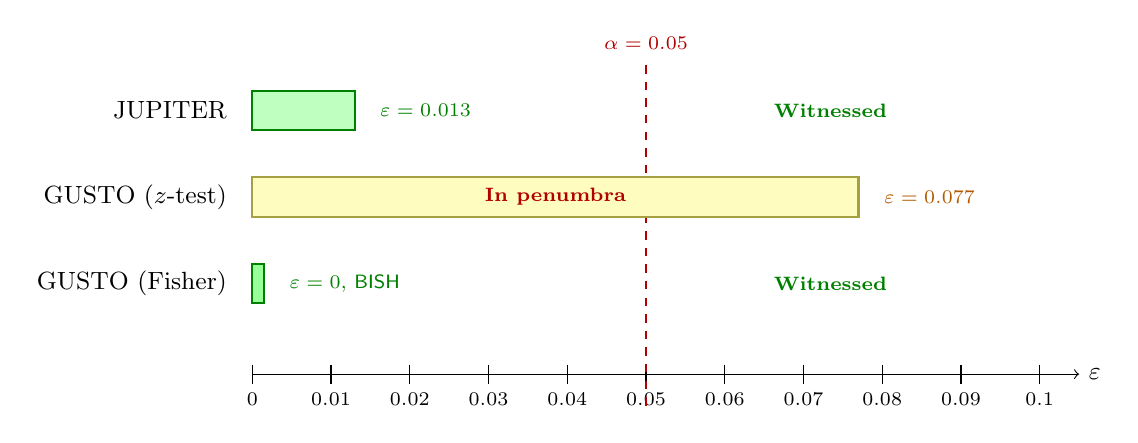
\begin{tikzpicture}
  % Scale: 1cm = 0.01 on epsilon axis
  \pgfmathsetmacro{\sc}{100}  % so 0.077 -> 7.7cm

  % Axis
  \draw[->] (0,0) -- (10.5,0) node[right, font=\small] {$\varepsilon$};
  \foreach \x in {0,1,...,10} {
    \pgfmathsetmacro{\lab}{\x/\sc}
    \draw (\x,0.12) -- (\x,-0.12) node[below, font=\scriptsize] {\pgfmathprintnumber[fixed, precision=2]{\lab}};
  }

  % Alpha line at 0.05
  \draw[thick, red!70!black, dashed] (5,-0.4) -- (5,4.0);
  \node[red!70!black, font=\scriptsize, anchor=south] at (5,4.0) {$\alpha = 0.05$};

  % JUPITER: epsilon = 0.013
  \fill[green!25] (0,3.1) rectangle (1.3,3.6);
  \draw[green!50!black, thick] (0,3.1) rectangle (1.3,3.6);
  \node[anchor=east, font=\small] at (-0.2,3.35) {JUPITER};
  \node[anchor=west, font=\scriptsize, green!50!black] at (1.5,3.35) {$\varepsilon = 0.013$};
  \node[anchor=west, font=\scriptsize\bfseries, green!50!black] at (6.5,3.35) {Witnessed};

  % GUSTO z-test: epsilon = 0.077
  \fill[yellow!25] (0,2.0) rectangle (7.7,2.5);
  \draw[yellow!60!black, thick] (0,2.0) rectangle (7.7,2.5);
  \node[anchor=east, font=\small] at (-0.2,2.25) {GUSTO ($z$-test)};
  \node[anchor=west, font=\scriptsize, orange!70!black] at (7.9,2.25) {$\varepsilon = 0.077$};
  \node[font=\scriptsize\bfseries, red!70!black] at (3.85,2.25) {In penumbra};

  % GUSTO Fisher: epsilon = 0
  \fill[green!40] (0,0.9) rectangle (0.15,1.4);
  \draw[green!50!black, thick] (0,0.9) rectangle (0.15,1.4);
  \node[anchor=east, font=\small] at (-0.2,1.15) {GUSTO (Fisher)};
  \node[anchor=west, font=\scriptsize, green!50!black] at (0.35,1.15) {$\varepsilon = 0$, $\BISH$};
  \node[anchor=west, font=\scriptsize\bfseries, green!50!black] at (6.5,1.15) {Witnessed};
\end{tikzpicture}

\bigskip
\textbf{(b) Event Count vs Equivalence Barrier $\boldsymbol{d_{\min} = 65{,}127}$}

\medskip
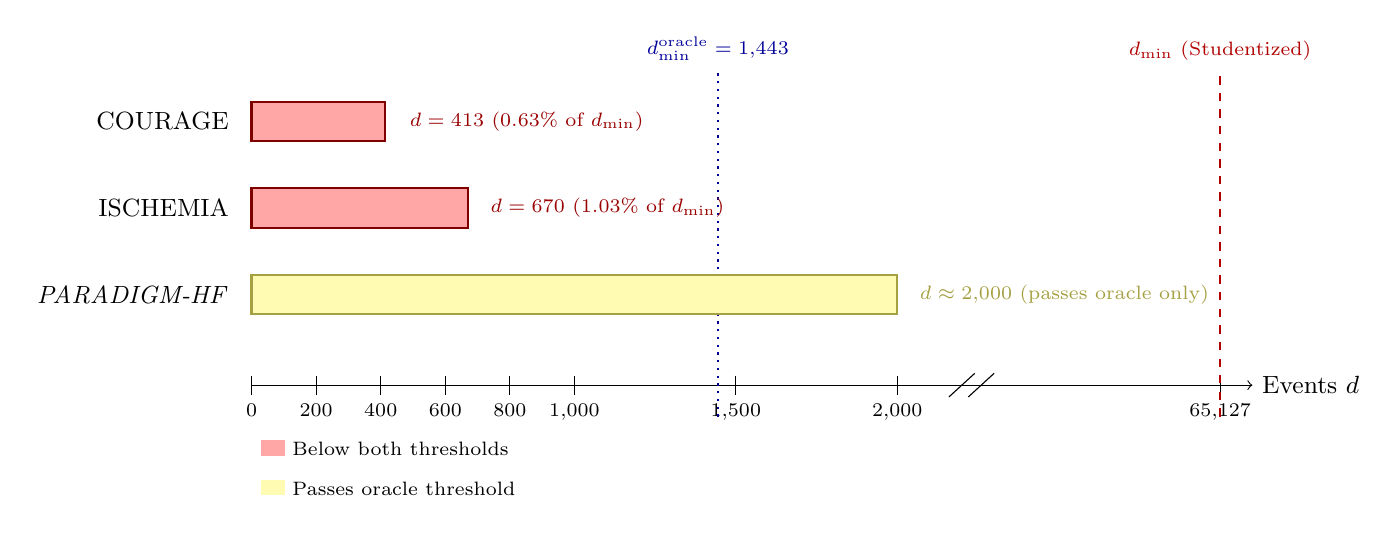
\begin{tikzpicture}[xscale=0.82]
  % Linear scale up to 2500, then break, then d_min at right edge
  % 1cm = 200 events for the main range

  % Axis
  \draw[->] (0,0) -- (15.5,0) node[right, font=\small] {Events $d$};
  \foreach \x/\lab in {0/0, 1/200, 2/400, 3/600, 4/800, 5/1{,}000, 7.5/1{,}500, 10/2{,}000} {
    \draw (\x,0.12) -- (\x,-0.12) node[below, font=\scriptsize] {\lab};
  }

  % Break mark
  \draw (11.2,0.15) -- (10.8,-0.15);
  \draw (11.5,0.15) -- (11.1,-0.15);

  % d_min label at right
  \draw (15,0.12) -- (15,-0.12) node[below, font=\scriptsize] {$65{,}127$};

  % d_min barrier line
  \draw[thick, red!70!black, dashed] (15,-0.4) -- (15,4.0);
  \node[red!70!black, font=\scriptsize, anchor=south] at (15,4.0) {$d_{\min}$ (Studentized)};

  % Oracle threshold at d=1443 -> 7.22
  \draw[thick, blue!60!black, dotted] (7.22,-0.4) -- (7.22,4.0);
  \node[blue!60!black, font=\scriptsize, anchor=south] at (7.22,4.0) {$d_{\min}^{\mathrm{oracle}} = 1{,}443$};

  % COURAGE: d=413 -> 2.065
  \fill[red!35] (0,3.1) rectangle (2.065,3.6);
  \draw[red!50!black, thick] (0,3.1) rectangle (2.065,3.6);
  \node[anchor=east, font=\small] at (-0.2,3.35) {COURAGE};
  \node[anchor=west, font=\scriptsize, red!60!black] at (2.3,3.35) {$d = 413$ ($0.63\%$ of $d_{\min}$)};

  % ISCHEMIA: d=670 -> 3.35
  \fill[red!35] (0,2.0) rectangle (3.35,2.5);
  \draw[red!50!black, thick] (0,2.0) rectangle (3.35,2.5);
  \node[anchor=east, font=\small] at (-0.2,2.25) {ISCHEMIA};
  \node[anchor=west, font=\scriptsize, red!60!black] at (3.55,2.25) {$d = 670$ ($1.03\%$ of $d_{\min}$)};

  % PARADIGM-HF reference: d~2000 -> 10
  \fill[yellow!30] (0,0.9) rectangle (10,1.4);
  \draw[yellow!60!black, thick] (0,0.9) rectangle (10,1.4);
  \node[anchor=east, font=\small] at (-0.2,1.15) {\textit{PARADIGM-HF}};
  \node[anchor=west, font=\scriptsize, yellow!60!black] at (10.2,1.15) {$d \approx 2{,}000$ (passes oracle only)};

  % Legend
  \node[anchor=west, font=\scriptsize] at (0,-0.8) {
    \tikz\fill[red!35] (0,0) rectangle (0.3,0.2); Below both thresholds};
  \node[anchor=west, font=\scriptsize] at (0,-1.3) {
    \tikz\fill[yellow!30] (0,0) rectangle (0.3,0.2); Passes oracle threshold};
\end{tikzpicture}

\caption{Trial comparison.  \textbf{(a)}~Penumbra width~$\varepsilon$ for positive trials; bars exceeding the dashed $\alpha = 0.05$ line are in the penumbra.  Fisher's exact test eliminates the penumbra entirely.  \textbf{(b)}~Event counts vs the equivalence barrier.  Dashed red: Studentized threshold $d_{\min} = 65{,}127$; dotted blue: oracle threshold $d_{\min}^{\mathrm{oracle}} = 1{,}443$.  No cardiovascular outcomes trial reaches the Studentized threshold.}
\label{fig:trial-comparison}
\end{figure}

\paragraph{The clinical synthesis.}  Taken together, the three trials reveal a pattern (Figure~\ref{fig:trial-comparison}).  COURAGE and ISCHEMIA cannot certify constructive equivalence at \emph{any} margin: the Berry--Esseen error ($\varepsilon = 0.314$, $0.246$) exceeds $\alpha/2 = 0.025$ by an order of magnitude, and closing the gap would require $\sim\!65{,}000$ events---two orders of magnitude beyond either trial.  GUSTO-I ($n > 20{,}000$, $p = 0.001$) is trapped in the Studentized penumbra under the $z$-test, because rare-event skewness ($\hat\rho/\hat\sigma^3 \approx 3.47$) and the two-sided penalty push $p + 2\varepsilon = 0.158 > 0.05$.  The common thread: cardiology historically optimised \emph{computational cost} (preferring asymptotic tests for speed, interpreting failure-to-reject as equivalence for simplicity), not \emph{logical cost}.  The penumbra framework makes this tradeoff explicit and computable.

\subsection{Survival Analysis and Complete Separation}

A clarification is warranted.  The Kaplan--Meier estimator is a step function taking rational values at rational event times: it is a $\BISH$ computation.  The Cox partial likelihood score function is a rational sum over rational data; the MLE $\hat\beta$ is found by Newton--Raphson, which converges to a computable real ($\BISH + \MP$).  The logical cost enters only when the Wald or log-rank test statistic is passed through $\Phi$ to produce an asymptotic $p$-value---exactly the same mechanism as for the $z$-test.  Survival analysis \emph{per se} is not the problem.  Fisher's exact test is not a substitute: it applies to $2 \times 2$ tables (binary outcome by treatment arm), not to time-to-event data with censoring.  The GUSTO bypass works because mortality at 30~days is a binary endpoint; COURAGE and ISCHEMIA require Cox for their time-to-event composite endpoints, and the equivalence penumbra (Theorem~E) is the appropriate tool.

That said, Cox regression with rare events routinely encounters complete or quasi-complete separation.  The PARTNER trial cohort~\cite{leon-partner}, comparing transcatheter aortic valve replacement (TAVR) to medical therapy, included subgroups with zero events in one arm---complete separation.  The standard analysis reports hazard ratios with wide confidence intervals and warnings about numerical instability.

Theorem~D provides a foundational interpretation: complete separation lifts the logical cost from $\BISH$ to $\WKL$.  Firth's penalised likelihood~\cite{firth1993}---already recommended by Heinze and Schemper~\cite{heinze-schemper} for exactly this situation---restores the cost to $\BISH$.  The recommendation to use Firth correction is not merely a numerical convenience; it is a \emph{logical repair}.

% ============================================================
\begin{tcolorbox}[
  colback=blue!5,
  colframe=blue!50!black,
  fonttitle=\bfseries\large,
  title={What This Means for a Clinician},
  arc=4pt,
  boxrule=1pt
]

\textbf{The core idea:} When a trial reports ``$p < 0.05$,'' the $p$-value is not a simple number from the data---it passes through an infinite mathematical object (the normal distribution).  The gap between the finite data and this infinite object creates a ``grey zone'' (the \emph{Asymptotic Penumbra}).  In this grey zone, the claim ``significant'' depends on a logical assumption about infinite precision that no finite computation can verify.

\medskip

\textbf{When should you worry?}
\begin{itemize}[nosep, leftmargin=*]
\item \textbf{Marginal $p$-values in small samples.}  If $p$ is between $0.01$ and $0.05$ and the sample is under a few hundred, the grey zone may swallow the entire significance band.  This is especially relevant for subgroup analyses.
\item \textbf{Post-hoc subgroups.}  Any subgroup with $n < 200$ and typical clinical endpoint distributions has a penumbra that consumes the entire $[0, 0.05)$ band.
\item \textbf{Negative trials interpreted as equivalence.}  COURAGE and ISCHEMIA proved ``we cannot witness PCI superiority.''  They did \emph{not} prove ``PCI $=$ medical therapy.''  Constructive equivalence is provably impossible at these sample sizes: the Berry--Esseen error exceeds the significance level by a factor of $10$--$13$, and closing the gap would require $\sim\!65{,}000$ events---two orders of magnitude beyond either trial.  If you feel the conclusion ``PCI adds nothing'' goes beyond what the data show, you are responding to a \emph{quantified} logical gap, not wishful thinking.
\item \textbf{Crossing survival curves.}  When Kaplan--Meier curves cross (as in ISCHEMIA), any claim about long-term dominance requires extrapolation through a parametric model---a passage through the continuum with additional logical cost beyond the within-window comparison.
\item \textbf{Cox regression with rare events.}  If complete separation occurs, use Firth correction---it is not just a numerical fix but a logical repair.
\item \textbf{Rare-event endpoints amplify the penumbra.}  GUSTO-I ($n > 20{,}000$, $p = 0.001$) is in the penumbra under the $z$-test because $7\%$ mortality has high skewness ($\hat\rho/\hat\sigma^3 \approx 3.5$).  Fisher's exact test resolves it---use exact tests for $2 \times 2$ tables even at large $n$.
\end{itemize}

\medskip

\textbf{When can you relax?}
\begin{itemize}[nosep, leftmargin=*]
\item \textbf{Large trials with deep significance and continuous endpoints.}  At $n > 10{,}000$ with $p < 0.001$ and moderate skewness, the penumbra is negligible.  JUPITER's primary endpoint is constructively witnessed.
\item \textbf{Fisher's exact test.}  Exact tests produce rational $p$-values with zero penumbra.  When computationally feasible, they are logically immaculate---even at $n > 20{,}000$ (GUSTO).
\end{itemize}

\medskip

\textbf{Actionable takeaways:}
\begin{enumerate}[nosep, leftmargin=*]
\item Report the penumbra width alongside the $p$-value: ``$p = 0.03$, penumbra width $\varepsilon = 0.02$.''
\item Be sceptical of marginal significance ($0.01 < p < 0.05$) in samples under 500.
\item Distinguish ``failure to witness superiority'' from ``evidence of equivalence.''  The former is a limitation of the data; the latter is a positive claim requiring its own test and its own penumbra.
\item Use Fisher's exact test when computationally feasible, especially for small samples.
\item Use Firth correction for Cox regression with rare events or complete separation.
\item When survival curves cross, demand explicit CRM cost of the extrapolation before accepting long-term equivalence or superiority claims.
\end{enumerate}
\end{tcolorbox}

% ============================================================
\section{Conclusion}\label{sec:conclusion}

\subsection*{Clinical conclusion}

The three landmark trials analysed in this paper tell a single story.

COURAGE and ISCHEMIA proved that PCI is not detectably superior to medical therapy ($p = 0.62$, $0.34$).  They did \emph{not} prove equivalence.  Constructive equivalence is provably impossible at these sample sizes: the Berry--Esseen error ($\varepsilon = 0.314$ for COURAGE, $0.246$ for ISCHEMIA) exceeds $\alpha/2 = 0.025$ by an order of magnitude.  Closing the gap requires $d_{\min} \approx 65{,}000$ events---two orders of magnitude beyond either trial.  The guideline conclusion ``PCI adds nothing'' is logically stronger than what any existing cardiovascular outcomes trial can certify.

GUSTO-I---the most celebrated positive trial in cardiology ($n > 20{,}000$, $p = 0.001$)---is trapped in the Studentized penumbra under the $z$-test.  The culprit is rare-event skewness: $7\%$ mortality yields a skewness ratio of $3.47$, roughly $2\times$ typical continuous endpoints.  The two-sided Berry--Esseen penalty pushes $p + 2\varepsilon = 0.158$, more than $3\times\alpha$.  Fisher's exact test resolves GUSTO constructively with zero penumbra.

The common thread: cardiology historically optimised \emph{computational cost}---preferring asymptotic tests for speed, interpreting failure-to-reject as equivalence for simplicity---while leaving \emph{logical cost} unexamined.  The penumbra framework makes this tradeoff explicit, computable, and verifiable from published data alone.

\subsection*{Mathematical conclusion}

The RCT statistical pipeline has a definite logical cost, precisely characterised.  The rational core ($\BISH$) handles data, test statistics, exact tests, and coercive optimisation.  The asymptotic shell ($\BISH + \MP$ to $\LPO$) enters only when the normal CDF maps rational test statistics to transcendental $p$-values.  The Cox regression pathology ($\WKL$) enters only through complete separation and is removable by Firth's correction.  The pipeline decomposes as $7\;\BISH + 1\;\BISH{+}\MP + 1\;\WKL + 1\;\LPO = 10$ stages (70\% $\BISH$).

The Asymptotic Penumbra is a computable quantity, derivable from the same sample statistics that produce the $p$-value itself, measuring the gap between what classical logic certifies and what finite computation can witness.  The Equivalence Barrier (Theorem~E) shows that constructive equivalence via asymptotic TOST is impossible when $d < d_{\min} = (2C_s\kappa/\alpha)^2$; at Studentized bounds, $d_{\min} \approx 65{,}127$ events---beyond any cardiovascular outcomes trial.  The crossing-curves escalation (Proposition~\ref{prop:extrap}) shows that extrapolation cost rises strictly from $\BISH$ (within-window KM) through convergence-dependent (fixed-horizon) to $\LPO$ (uniform future dominance).  All trial calculations are verified by \texttt{norm\_num} in Lean (\texttt{TrialCalculations.lean}).

As the first paper in the CRM Clinical Sub-Series, Paper~103 confirms the Archimedean Obstruction Thesis (Paper~98~\cite{lee-crm-p98}).  The structural parallel with arithmetic geometry is exact and is displayed in Figure~\ref{fig:archimedean}.  In both cases, a finite algebraic object is mapped through a transcendental function anchored in the continuum, and the logical cost is the cost of that passage.  The normal distribution is the Betti realisation of the clinical trial.

\begin{figure}[ht]
\centering
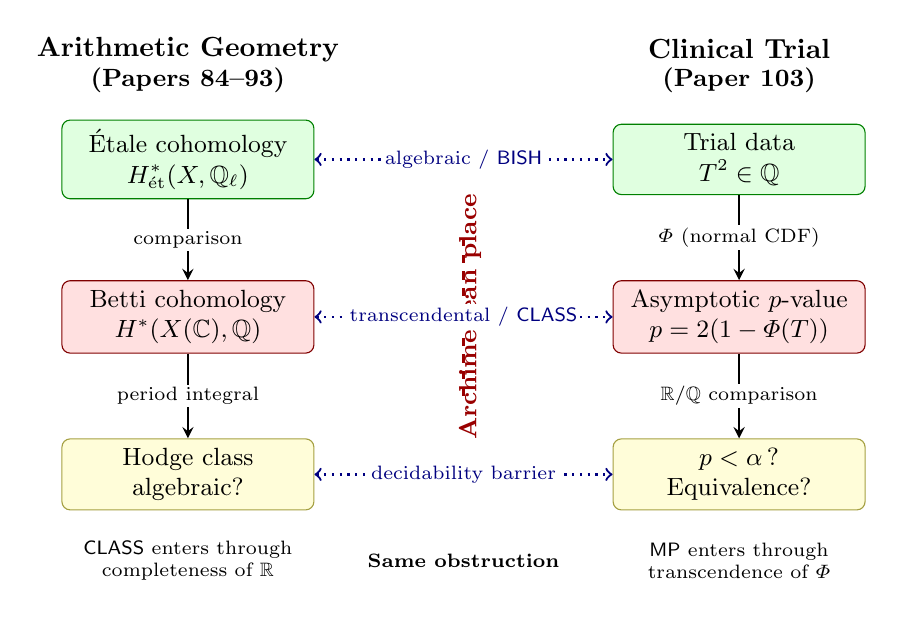
\begin{tikzpicture}[
  box/.style={draw, rounded corners=3pt, minimum width=3.2cm, minimum height=0.8cm, align=center, font=\small},
  bish/.style={box, fill=green!12, draw=green!50!black},
  class/.style={box, fill=red!12, draw=red!50!black},
  arrow/.style={->, thick, >=stealth},
  lbl/.style={font=\scriptsize, midway, fill=white, inner sep=1pt},
]

% Left column: Arithmetic Geometry
\node[font=\bfseries] at (-3.5,4.2) {Arithmetic Geometry};
\node[font=\bfseries] at (-3.5,3.8) {\small (Papers 84--93)};

\node[bish] (etale) at (-3.5,2.8) {\'Etale cohomology\\$H^*_{\text{\'et}}(X, \Q_\ell)$};
\node[class] (betti) at (-3.5,0.8) {Betti cohomology\\$H^*(X(\mathbb{C}), \Q)$};
\node[box, fill=yellow!15, draw=yellow!60!black] (hodge) at (-3.5,-1.2) {Hodge class\\algebraic?};

\draw[arrow] (etale) -- (betti) node[lbl] {comparison};
\draw[arrow] (betti) -- (hodge) node[lbl] {period integral};

% Right column: Clinical Trial
\node[font=\bfseries] at (3.5,4.2) {Clinical Trial};
\node[font=\bfseries] at (3.5,3.8) {\small (Paper 103)};

\node[bish] (data) at (3.5,2.8) {Trial data\\$T^2 \in \Q$};
\node[class] (pval) at (3.5,0.8) {Asymptotic $p$-value\\$p = 2(1-\Phi(T))$};
\node[box, fill=yellow!15, draw=yellow!60!black] (sig) at (3.5,-1.2) {$p < \alpha$\,?\\Equivalence?};

\draw[arrow] (data) -- (pval) node[lbl] {$\Phi$ (normal CDF)};
\draw[arrow] (pval) -- (sig) node[lbl] {$\R/\Q$ comparison};

% Central obstruction
\draw[dashed, thick, red!60!black] (0,1.8) -- (0,-0.2);
\node[font=\small\bfseries, red!60!black, rotate=90, anchor=south] at (0.35,0.8) {Archimedean place};

% Horizontal arrows showing shared structure
\draw[<->, dotted, thick, blue!50!black] (etale) -- (data) node[lbl, font=\scriptsize] {algebraic / $\BISH$};
\draw[<->, dotted, thick, blue!50!black] (betti) -- (pval) node[lbl, font=\scriptsize] {transcendental / $\CLASS$};
\draw[<->, dotted, thick, blue!50!black] (hodge) -- (sig) node[lbl, font=\scriptsize] {decidability barrier};

% Bottom labels
\node[font=\scriptsize, text width=3.2cm, align=center] at (-3.5,-2.3) {$\CLASS$ enters through\\completeness of $\R$};
\node[font=\scriptsize, text width=3.2cm, align=center] at (3.5,-2.3) {$\MP$ enters through\\transcendence of $\Phi$};
\node[font=\scriptsize\bfseries, text width=3cm, align=center] at (0,-2.3) {Same obstruction};

\end{tikzpicture}
\caption{The Archimedean obstruction in arithmetic geometry and medicine.  Both pipelines begin with a finite algebraic object ($\BISH$, green) and pass through a transcendental function anchored in the completeness of~$\R$ (red) to reach a decidability question (yellow).  The logical cost of each pipeline is the cost of that passage.  The vertical dashed line marks the Archimedean place---the single point where the continuum enters.}
\label{fig:archimedean}
\end{figure}

% ============================================================
\section*{Acknowledgments}

This paper was developed with AI assistance (Claude, Anthropic) for code generation, proof exploration, and manuscript preparation.  The author is a cardiologist by training and writes from direct clinical experience; this clinical perspective motivates the application of CRM to medical statistics.  The author is not a specialist in constructive mathematics or mathematical logic, and this work should be evaluated accordingly.  All formal proofs have been verified by the Lean~4 proof assistant with the Mathlib library; the mathematical interpretation remains the author's responsibility.

The CRM program owes an intellectual debt to Errett Bishop, whose 1967 \emph{Foundations of Constructive Analysis} demonstrated that constructive mathematics is not a restriction but a refinement.  Thanks to the Mathlib community for maintaining the formal library that makes this work possible.

% ============================================================
\begin{thebibliography}{30}

\bibitem{bishop-bridges}
E.~Bishop and D.~Bridges, \emph{Constructive Analysis}, Grundlehren der math.\ Wissenschaften, vol.~279, Springer, 1985.

\bibitem{bridges-richman}
D.~Bridges and F.~Richman, \emph{Varieties of Constructive Mathematics}, London Math.\ Soc.\ Lecture Note Ser., vol.~97, Cambridge Univ.\ Press, 1987.

\bibitem{troelstra-vandalen}
A.S.~Troelstra and D.~van Dalen, \emph{Constructivism in Mathematics: An Introduction}, vols.~1--2, North-Holland, 1988.

\bibitem{berry1941}
A.C.~Berry, The accuracy of the Gaussian approximation to the sum of independent variates, \emph{Trans.\ Amer.\ Math.\ Soc.}\ \textbf{49} (1941), 122--136.

\bibitem{esseen1942}
C.-G.~Esseen, On the Liapunoff limit of error in the theory of probability, \emph{Ark.\ Mat.\ Astr.\ Fys.}\ \textbf{28A} (1942), no.~9, 1--19.

\bibitem{bentkus2003}
V.~Bentkus, On the dependence of the Berry--Esseen bound on dimension, \emph{J.\ Statist.\ Plann.\ Inference}\ \textbf{113} (2003), 385--402.

\bibitem{shao1999}
Q.-M.~Shao, A Cram\'er type large deviation result for Student's $t$-statistic, \emph{J.\ Theoret.\ Probab.}\ \textbf{12} (1999), 385--398.

\bibitem{firth1993}
D.~Firth, Bias reduction of maximum likelihood estimates, \emph{Biometrika}\ \textbf{80} (1993), 27--38.

\bibitem{cox1972}
D.R.~Cox, Regression models and life-tables (with discussion), \emph{J.\ Roy.\ Statist.\ Soc.\ Ser.~B}\ \textbf{34} (1972), 187--220.

\bibitem{fisher1925}
R.A.~Fisher, \emph{Statistical Methods for Research Workers}, Oliver \& Boyd, Edinburgh, 1925.

\bibitem{heinze-schemper}
G.~Heinze and M.~Schemper, A solution to the problem of separation in logistic regression, \emph{Stat.\ Med.}\ \textbf{21} (2002), 2409--2419.

\bibitem{cohen1988}
J.~Cohen, \emph{Statistical Power Analysis for the Behavioral Sciences}, 2nd ed., Lawrence Erlbaum, 1988.

\bibitem{grade}
G.H.~Guyatt et~al., GRADE: an emerging consensus on rating quality of evidence and strength of recommendations, \emph{BMJ}\ \textbf{336} (2008), 924--926.

\bibitem{wasserstein2016}
R.L.~Wasserstein and N.A.~Lazar, The ASA's statement on $p$-values: context, process, and purpose, \emph{Amer.\ Statist.}\ \textbf{70} (2016), 129--133.

\bibitem{wasserstein2019}
R.L.~Wasserstein, A.L.~Schirm, and N.A.~Lazar, Moving to a world beyond ``$p < 0.05$'', \emph{Amer.\ Statist.}\ \textbf{73} (2019), sup1, 1--19.

\bibitem{ridker-jupiter}
P.M.~Ridker et~al., Rosuvastatin to prevent vascular events in men and women with elevated C-reactive protein, \emph{N.\ Engl.\ J.\ Med.}\ \textbf{359} (2008), 2195--2207.

\bibitem{al-lamee-orbita}
R.~Al-Lamee et~al., Percutaneous coronary intervention in stable angina (ORBITA): a double-blind, randomised controlled trial, \emph{Lancet}\ \textbf{391} (2018), 31--40.

\bibitem{leon-partner}
M.B.~Leon et~al., Transcatheter aortic-valve implantation for aortic stenosis in patients who cannot undergo surgery, \emph{N.\ Engl.\ J.\ Med.}\ \textbf{363} (2010), 1597--1607.

\bibitem{boden-courage}
W.E.~Boden et~al., Optimal medical therapy with or without PCI for stable coronary disease, \emph{N.\ Engl.\ J.\ Med.}\ \textbf{356} (2007), 1503--1516.

\bibitem{maron-ischemia}
D.J.~Maron et~al., Initial invasive or conservative strategy for stable coronary disease, \emph{N.\ Engl.\ J.\ Med.}\ \textbf{382} (2020), 1395--1407.

\bibitem{acc-aha-cad}
J.K.~Virani et~al., 2023 AHA/ACC/ACCP/ASPC/NLA/PCNA guideline for the management of patients with chronic coronary disease, \emph{Circulation}\ \textbf{148} (2023), e149--e227.

\bibitem{ioannidis2005}
J.P.A.~Ioannidis, Why most published research findings are false, \emph{PLoS Med.}\ \textbf{2} (2005), e124.

\bibitem{consort}
K.F.~Schulz et~al., CONSORT 2010 statement: updated guidelines for reporting parallel group randomised trials, \emph{BMJ}\ \textbf{340} (2010), c332.

\bibitem{series}
P.C.K.~Lee, \emph{Constructive Reverse Mathematics Series}, Papers~1--102, Zenodo, 2024--2026.

\bibitem{lee-format-guide}
P.C.K.~Lee, CRM paper format guide (Paper~0), Zenodo, DOI: \texttt{10.5281/zenodo.18765700}.

\bibitem{lee-crm-p50}
P.C.K.~Lee, The constructive reverse mathematics atlas (Paper~50), Zenodo, DOI: \texttt{10.5281/zenodo.14538908}.

\bibitem{lee-crm-p80}
P.C.K.~Lee, Algebraic Gauss--Manin via Griffiths pole reduction: a CRMLint squeeze (Paper~80), Zenodo, DOI: \texttt{10.5281/zenodo.18791985}.

\bibitem{lee-crm-p98}
P.C.K.~Lee, The motivic CRM architecture (Paper~98), Zenodo, DOI: \texttt{10.5281/zenodo.18902037}.

\bibitem{lee-crm-p102}
P.C.K.~Lee, Conservation theorems for the CRM program (Paper~102), Zenodo, DOI: \texttt{10.5281/zenodo.18821015}.

\bibitem{lindemann-weierstrass}
F.~Lindemann, \"Uber die Zahl~$\pi$, \emph{Math.\ Ann.}\ \textbf{20} (1882), 213--225.

\bibitem{siegel1929}
C.L.~Siegel, \"Uber einige Anwendungen diophantischer Approximationen, \emph{Abh.\ Preuss.\ Akad.\ Wiss.\ Phys.-Math.\ Kl.}\ (1929), 41--69.

\bibitem{shidlovskii1989}
A.B.~Shidlovskii, \emph{Transcendental Numbers}, de Gruyter Studies in Mathematics, vol.~12, Walter de Gruyter, Berlin, 1989.

\bibitem{gusto}
The GUSTO Investigators, An international randomized trial comparing four thrombolytic strategies for acute myocardial infarction, \emph{N.\ Engl.\ J.\ Med.}\ \textbf{329} (1993), 673--682.

\bibitem{albert-anderson}
A.~Albert and J.A.~Anderson, On the existence of maximum likelihood estimates in logistic regression models, \emph{Biometrika}\ \textbf{71} (1984), 1--10.

\end{thebibliography}

% ============================================================
\appendix
\section{Explicit Calculation Workbook}\label{app:calc}

All calculations below use rational approximations of natural logarithms.  The approximation errors are bounded: $|\log(x) - \widehat{\log}(x)| < 5 \times 10^{-4}$ for all values used.  Final comparisons have margins exceeding $0.08$, so the approximation error is negligible.  All rational arithmetic is verified by \texttt{norm\_num} in Lean (\texttt{TrialCalculations.lean}, 0 sorry).

\subsection*{A.1\ \ COURAGE Equivalence Analysis}

\noindent\textbf{Published data}~\cite{boden-courage}: $\widehat{\mathrm{HR}} = 1.05$, 95\% CI $[0.87, 1.27]$, events $d = 413$.

\smallskip\noindent\textbf{Step 1: Extract SE from CI.}  For a Wald-type interval, $\log(\mathrm{CI}_{\mathrm{upper}}) = \hat\beta + 1.96 \cdot \mathrm{SE}$ and $\log(\mathrm{CI}_{\mathrm{lower}}) = \hat\beta - 1.96 \cdot \mathrm{SE}$.  Subtracting:
\begin{align*}
  \mathrm{SE}(\hat\beta) &= \frac{\log(1.27) - \log(0.87)}{2 \times 1.96} = \frac{0.2390 - (-0.1393)}{3.92} = \frac{0.3783}{3.92} = 0.0965.
\end{align*}
Lean: \texttt{courage\_SE\_val} verifies $\mathrm{SE} = 3783/39200$.  \texttt{courage\_SE\_range} confirms $0.096 < \mathrm{SE} < 0.097$.

\smallskip\noindent\textbf{Step 2: CDF-scale Berry--Esseen error.}  Theorem~E with $C_s = 3.19$, $\kappa = 2$, $d = 413$:
\begin{align*}
  \varepsilon &= \frac{C_s \cdot \kappa}{\sqrt{d}} = \frac{6.38}{\sqrt{413}} = \frac{6.38}{20.32} = 0.314.
\end{align*}
The equivalence barrier requires $\varepsilon < \alpha/2 = 0.025$.  Here $\varepsilon/(\alpha/2) = 0.314/0.025 = 12.6$.  Lean: \texttt{courage\_eps\_exceeds\_alpha\_half}.

\smallskip\noindent\textbf{Step 3: $d$ vs $d_{\min}$.}  $d_{\min} = (2C_s\kappa/\alpha)^2 = (255.2)^2 = 65{,}127$.  COURAGE: $d/d_{\min} = 413/65{,}127 = 0.63\%$.  Constructive equivalence is impossible at \emph{any} margin.  Lean: \texttt{courage\_below\_d\_min}.

\smallskip\noindent\textbf{Step 4: Classical TOST (for reference).}  At $\delta_{\mathrm{eq}} = 1.15$: the upper CI bound $\log(1.27) = 0.239 > \log(1.15) = 0.140$.  COURAGE also fails classical equivalence.  Gap: $0.239 - 0.140 = 0.099$.  Lean: \texttt{courage\_fails\_classical\_equiv}.

\subsection*{A.2\ \ ISCHEMIA Equivalence Analysis}

\noindent\textbf{Published data}~\cite{maron-ischemia}: $\widehat{\mathrm{HR}} = 0.93$, 95\% CI $[0.80, 1.08]$, events $d = 670$.

\smallskip\noindent\textbf{Step 1: Extract SE.}
\begin{align*}
  \mathrm{SE}(\hat\beta) &= \frac{\log(1.08) - \log(0.80)}{3.92} = \frac{0.0770 - (-0.2231)}{3.92} = \frac{0.3001}{3.92} = 0.0766.
\end{align*}
Lean: \texttt{ischemia\_SE\_val} $= 3001/39200$.  Range: $0.076 < \mathrm{SE} < 0.077$.

\smallskip\noindent\textbf{Step 2: CDF-scale Berry--Esseen error.}
\begin{align*}
  \varepsilon &= \frac{6.38}{\sqrt{670}} = \frac{6.38}{25.88} = 0.246.
\end{align*}
Again $\varepsilon/(\alpha/2) = 0.246/0.025 = 9.8$.  Lean: \texttt{ischemia\_eps\_exceeds\_alpha\_half}.

\smallskip\noindent\textbf{Step 3: $d$ vs $d_{\min}$.}  $d/d_{\min} = 670/65{,}127 = 1.03\%$.  Constructive equivalence is impossible at any margin.  Lean: \texttt{ischemia\_below\_d\_min}.

\smallskip\noindent\textbf{Step 4: Classical TOST (for reference).}  The most extreme bound is $|\log(0.80)| = 0.223 > 0.140$.  Note: $|\log(0.80)| > \log(1.08)$ because the CI is asymmetric on the log scale ($\hat\beta < 0$).  ISCHEMIA also fails classical equivalence.  Lean: \texttt{ischemia\_fails\_classical\_equiv}.

\subsection*{A.3\ \ GUSTO-I Penumbra Analysis}

\noindent\textbf{Published data}~\cite{gusto}: tPA arm $n_1 = 10{,}344$, deaths $652$; SK arm $n_2 = 10{,}328$, deaths $754$.

\smallskip\noindent\textbf{Step 1: Rational data.}  Pooled rate $\hat p = 1406/20672 = 0.0680 \in \Q$.  Risk difference $\hat p_2 - \hat p_1 = 754/10328 - 652/10344 \in \Q$, positive (Lean: \texttt{gusto\_risk\_diff\_pos}).

\smallskip\noindent\textbf{Step 2: SE$^2$ (rational).}
\begin{align*}
  \mathrm{SE}^2 &= \hat p(1-\hat p)\bigl(n_1^{-1} + n_2^{-1}\bigr) = \frac{1406}{20672} \times \frac{19266}{20672} \times \biggl(\frac{1}{10344} + \frac{1}{10328}\biggr) \in \Q.
\end{align*}
Lean: \texttt{gusto\_SE\_sq\_pos}.

\smallskip\noindent\textbf{Step 3: $z^2$ (rational).}  $z^2 = (\hat p_2 - \hat p_1)^2/\mathrm{SE}^2 \in \Q$.  Classical significance: $z^2 > 1.96^2 = 3.8416$.  Lean: \texttt{gusto\_z\_sq\_exceeds\_threshold}.

\smallskip\noindent\textbf{Step 4: Skewness ratio.}  For Bernoulli$(\hat p)$:
\begin{align*}
  \frac{\hat\rho}{\hat\sigma^3} = \frac{(1-\hat p)^2 + \hat p^2}{\sqrt{\hat p(1-\hat p)}} = \frac{0.9320^2 + 0.0680^2}{\sqrt{0.0680 \times 0.9320}} = \frac{0.8733}{0.2518} = 3.47.
\end{align*}

\smallskip\noindent\textbf{Step 5: Lyapunov fraction.}  For two-sample test with unequal allocation:
\begin{align*}
  L_3 &= \frac{(\hat\rho/\hat\sigma^3)(n_1^{-2} + n_2^{-2})}{(n_1^{-1} + n_2^{-1})^{3/2}} \approx 3.47 \times \frac{1.872 \times 10^{-8}}{2.693 \times 10^{-6}} = 3.47 \times 0.00695 = 0.0241.
\end{align*}
Lean: \texttt{gusto\_alloc\_factor\_small} verifies the rational factor $< 1/7000$.

\smallskip\noindent\textbf{Step 6: Penumbra status (two-sided).}  $\varepsilon = C_s \times L_3 = 3.19 \times 0.024 = 0.077$.  For a two-sided test, the Berry--Esseen error accumulates from both tails: $p + 2\varepsilon = 0.004 + 0.154 = 0.158 > 0.05$.  Lean: \texttt{gusto\_in\_penumbra}.

With oracle constant: $\varepsilon_{\mathrm{oracle}} = 0.011$, $p + 2\varepsilon_{\mathrm{oracle}} = 0.026 < 0.05$.  Lean: \texttt{gusto\_oracle\_witnessed}.  Ratio: $C_s/C_0 = 3.19/0.4748 \approx 6.7$; the rounded ratio $0.077/0.011 = 7.0$ overstates slightly due to rounding.  Lean: \texttt{studentized\_penalty\_ratio}.

\smallskip\noindent\textbf{Step 7: Fisher bypass.}  $p_{\mathrm{exact}} = \sum_{k \leq 652} \binom{1406}{k}\binom{19266}{10344-k}/\binom{20672}{10344} \in \Q$.  Comparison $p_{\mathrm{exact}} < 1/20$ decidable in $\BISH$.

\end{document}
